% REMEMBER: You must not plagiarise anything in your report. Be extremely careful.
\documentclass{l4proj}

    
%==============================================================================
% Put any additional packages here
% You can add any packages you want, as long as it does not alter
% the overall format (e.g. don't change the margins or the reference style).
%
\usepackage{pdfpages} % if you want to include a PDF for an ethics checklist, for example
\usepackage{enumitem}
%
%

\begin{document}

%==============================================================================
%% METADATA
\title{Seminar Roulette: An Event Recommendation Platform for University Academics}
\author{Ollie Gardner}
\date{\today}

\maketitle

%==============================================================================
%% ABSTRACT
\begin{abstract}

The University of Glasgow does not offer a software solution that adopts a unified approach to seminar organisation and management. Current systems are ineffective in aiding time-poor academics to find new research seminars that they have not thought about attending before. Furthermore, current platforms do not include any personalised recommendation features. Seminar Roulette is a new web-based platform that scrapes seminar data from various University of Glasgow event feeds. It utilises an algorithmic recommender system to provide academics with personalised seminar suggestions based on how they have rated seminars that they have previously attended. An extensive evaluation was conducted, and it was concluded that Seminar Roulette effectively provides highly valuable event recommendations to members of the University of Glasgow academic community.

\end{abstract}

%==============================================================================
%% ACKNOWLEDGEMENTS
\chapter*{Acknowledgements}

I would like to thank my supervisor, Dr Jeremy Singer, for his guidance and support throughout the duration of this work. I would also like to thank the participants who completed my user evaluations as without them, this project would not have been possible.

%==============================================================================

% EDUCATION REUSE CONSENT FORM
% If you consent to your project being shown to future students for educational purposes
% then insert your name and the date below to  sign the education use form that appears in the front of the document. 
% You must explicitly give consent if you wish to do so.
% If you sign, your project may be included in the Hall of Fame if it scores particularly highly.
%
% Please note that you are under no obligation to sign 
% this declaration, but doing so would help future students.
%
\def\consentname {Ollie Gardner} % your full name
\def\consentdate {\today} % the date you agree
%
\educationalconsent


%==============================================================================
\tableofcontents

%==============================================================================
%% Notes on formatting
%==============================================================================
% The first page, abstract and table of contents are numbered using Roman numerals and are not
% included in the page count. 
%
% From now on pages are numbered
% using Arabic numerals. Therefore, immediately after the first call to \chapter we need the call
% \pagenumbering{arabic} and this should be called once only in the document. 
%
% Do not alter the bibliography style.
%
% The first Chapter should then be on page 1. You are allowed 40 pages for a 40 credit project and 30 pages for a 
% 20 credit report. This includes everything numbered in Arabic numerals (excluding front matter) up
% to but excluding the appendices and bibliography.
%
% You must not alter text size (it is currently 10pt) or alter margins or spacing.
%
%
%==================================================================================================================================
%
% IMPORTANT
% The chapter headings here are **suggestions**. You don't have to follow this model if
% it doesn't fit your project. Every project should have an introduction and conclusion,
% however. 
%
%==================================================================================================================================
\chapter{Introduction}

% reset page numbering. Don't remove this!
\pagenumbering{arabic}

This chapter will introduce the Seminar Roulette project. It will investigate the need for a web-based platform that enables members of the University of Glasgow academic community to discover research seminars that they are unaware of. Subsequent chapters in this paper will document the project's background, requirements, design, implementation, evaluation and conclusion.

\section{Motivation}
\label{section:motivation}

Every week, the University of Glasgow host an average of 15.4 (std. dev. 2.7, 169 seminars) research seminars that are attended by staff and students (see Figure \ref{fig:semester_2_seminars}). Due to the nature of their work, seminar attendees are time-poor and do not want the hassle of trawling through lists of events to find the ones which are of interest to them. Academics are often unsure if a seminar will be of interest to them or not, so they will choose not to attend. Furthermore, their diary schedule changes frequently, making it difficult to commit to the same seminars each week.

\begin{figure}[htb]
    \centering
    \includegraphics[width=0.6\linewidth]{images/semester_2_seminars.pdf}    
    \caption{A column chart showing the number of research seminars taking place each week at the University of Glasgow during semester two of session 2020/2021.}
    \label{fig:semester_2_seminars} 
\end{figure}

Currently, seminars and events at the University of Glasgow are advertised through various platforms. The most popular of these sources being; Samoa Events \citep{samoa}, Eventbrite \citep{eventbrite} and the University of Glasgow website \citep{uofg}. These systems will be analysed in-depth in Chapter \ref{chapter:background}. By having a mix of both internal and external sources, it can be an unattractive prospect for academics to spend the time to find a seminar that is of interest to them. They also must ensure that it fits around their timetable. User interaction with advertised events on the aforementioned platforms is minimal, so their feature sets are limited. For example, there is no way for academics to rate a seminar for other people to see. Furthermore, Samoa Events and the University's website do not offer personalised recommendations to users that are tailored towards their interests.

Recognising that an opportunity exists for a system that adopts a unified approach to seminar management, the prospect of a new application can start to be envisaged. This development will overcome the weaknesses of the platforms currently accessible to academics. Additional functionality will be added to the application which is presently unavailable on a University of Glasgow platform. There is potential for the new system to become a staple piece of software in the University's seminar community and be rolled out campus-wide. 

\section{Aims}
\label{sec:aims}

This project proposes Seminar Roulette, a new web-based platform that will allow University academics to discover research seminars that are of interest to them. The web application will be accessible to the whole University community and it endeavours to become the centralised source for seminar information. By being available to the entirety of the University, the system must support various types of users - staff members, students and researchers.

Seminar Roulette intends to provide academics with the ability to view events taking place at the University through one portal without having to browse various different websites. They will be able to login to the system using the University's single sign-on service, Shibboleth \citep{shibboleth}. Users will be able to enter their personal interests and rate seminars that they have previously attended. In response, Seminar Roulette will present them with recommendations based on past seminars which they have rated highly. Furthermore, a seminar's description will be analysed, with high-frequency words extracted, forming a set of keywords. These words will then be matched up with a user's interests using an algorithmic recommender system.

Requirement elicitation will be carried out using a survey sent out to a subset of staff members and students. In particular, the questionnaire will target those who regularly attend seminars to build a picture of what is missing within the event platforms currently available. Seminar Roulette should be responsive and able to be used without any prior training. It should have a visually pleasing user interface in order to drive user engagement with the system. High uptake with the platform will result in users benefiting from highly valuable seminar recommendations. To ensure Seminar Roulette is accessible to the whole University community, the application should be responsive to mobile and tablets whilst having the same feature set as desktop devices. Enabling the system to be accessible on any device will result in users being able to find seminar events whilst on the move. The sole deliverable of this project will be a web application hosted on a virtual machine and accessible via a domain name using any web browser.

Before the development of this project can begin, various preliminary stages need to be conducted, including; a period of initial requirement gathering with avid seminar attendees, establishing the core functional and non-functional requirements of the application and creating initial paper prototypes for the user interface. Following this introductory stage of the project, the software implementation will begin using a set of modern technologies that will allow for the group of requirements to be achieved. Finally, the usability and suitability of Seminar Roulette will be assessed through a questionnaire. The evaluation will collect two types of data - quantitative and qualitative. Quantitative data will be gathered through a Post-Study System Usability Questionnaire (PSSUQ) and will measure the end users' perceived satisfaction with the platform. Ideas of how Seminar Roulette could be improved in future iterations will be evaluated using five open-ended questions.

\section{Summary}

This chapter has introduced the motivation and aims of Seminar Roulette, comparing the project proposal with pre-existing services available to the University of Glasgow community. This paper will go on to outline how the motivation behind the project was developed into a working prototype. The subsequent chapters in this dissertation are structured as follows:

\begin{itemize}
    \item \textbf{Chapter 2} discusses how recommender systems are used within society. It also examines and compares pre-existing related seminar products, identifying their weaknesses and how they differ from Seminar Roulette.
    \item \textbf{Chapter 3} outlines the requirement gathering process and analyses the findings to build a set of functional and non-functional requirements.
    \item \textbf{Chapter 4} explains the design process, highlighting how Seminar Roulette was constructed. Furthermore, each design decision will be explored in-depth to ensure that it links back to the project requirements devised in Chapter \ref{chapter:requirements}.
    \item \textbf{Chapter 5} describes the methods used to build and implement the project and explores the software engineering techniques utilised to ensure effective and timely delivery of the end product. 
    \item \textbf{Chapter 6} details the processes carried out to evaluate the system, including; unit testing, system performance, two end-user evaluations and requirement validation.
    \item \textbf{Chapter 7} begins with a reflection of the overall success of Seminar Roulette. Next, the potential for future work and enhancements is discussed, and the paper concludes with a summary of the project's findings.
\end{itemize}


%==================================================================================================================================
\chapter{Background}
\label{chapter:background}

This chapter will discuss the project's background, examining how algorithmic recommender systems are used within popular e-commerce platforms. Following this, related products will be investigated, reviewing the drawbacks of these applications and how the new system will overcome them. Both internal and external software solutions to the University will be considered so that the aims set out in Section \ref{sec:aims} can be achieved.

\section{Recommender Systems in E-Commerce}

The e-commerce industry is growing by 23\% every year, attracting billions of monthly customers \citep{ecommercestats}. It is common for users of these platforms to become susceptible to information overload. Recommender systems overcome this issue through the use of custom user experience by searching through dynamically constructed data to display personalised content \citep{ISINKAYE2015261}.

In Sections \ref{section:netflix} and \ref{section:amazon}, Netflix and Amazon will act as case studies of e-commerce companies that utilise recommender system algorithms within their platforms. The products will be analysed, showing the different techniques of providing recommendations and how they can be applied to Seminar Roulette to enable academia to benefit from recommendation engines.

\subsection{Netflix}
\label{section:netflix}

As of 2020, Netflix has over 203 million paid subscribers, making it one of the largest streaming platforms in the world \citep{netflixstats}. A key feature of Netflix is their recommender system which allows their members to find videos to watch which they have not seen before. Research conducted by Netflix in 2016 revealed that people lose interest in films and TV shows after just 60 to 90 seconds after looking at anywhere between 10 and 20 shows \citep{10.1145/2843948}. Recommendation is so vital to Netflix that in October 2006, they released a data set containing 100 million movie ratings and tasked the world with developing an algorithm that could beat the accuracy of its own \citep{Bennett07thenetflix}. If anyone could develop such a system, there was a million-dollar prize to be won.

Netflix implement multiple strategies for recommending movies to their customers, nicknamed; \emph{Personalised Video Ranker}, \emph{Top-N Video Ranker} and \emph{Video-Video Similarity} \citep{10.1145/2843948}. The most noteworthy of these is their \emph{Personalised Video Ranker}  algorithm which uses item-based collaborative filtering to provide recommendations. This technique is used for the content which cannot be described by metadata. A database of user ratings is created, turned into a user-item matrix and similarities between user ratings are calculated to make movie recommendations \citep{ISINKAYE2015261}. A high-level representation of item-based collaborative filtering is pictured in Figure \ref{fig:item_based_filtering}.

Due to the new platform being similar to Netflix but using events instead of movies and TV shows, item-based collaborative filtering could be applied to give academics a personalised experience on the site. It is a tried and tested method that will result in Seminar Roulette providing valuable seminar recommendations to its users. 

\begin{figure}[htb] 
    \centering
    \begin{subfigure}[b]{0.42\textwidth}
        \includegraphics[width=\textwidth]{images/user_based_filtering.pdf}
        \caption{User-based filtering.}
        \label{fig:user_based_filtering}
    \end{subfigure}
    ~
    \begin{subfigure}[b]{0.42\textwidth}
        \includegraphics[width=\textwidth]{images/item_based_filtering.pdf}
        \caption{Item-based filtering.}
        \label{fig:item_based_filtering}
    \end{subfigure}
    ~
    \caption{Pictorial representation of user and item-based collaborative filtering using people and food. \subref{fig:user_based_filtering} shows user-based filtering - Tim's food choices have been recommended to John as they have both rated other foods similarly. \subref{fig:item_based_filtering} shows item-based filtering - an ice cream sundae has been recommended to John because he likes an ice cream cone. Figures adapted from \cite{uservsitemfiltering}.}
    \label{fig:collaborative_filtering}
\end{figure}

\subsection{Amazon}
\label{section:amazon}

Amazon's website attracts 2.5 billion monthly visitors \citep{ecommercestats} and as a result, the company has become well known for its personalisation features. The functionality has been a staple in Amazon's user experience for over two decades, resulting in every user viewing the platform differently. In 1998, Amazon released its item-based collaborative filtering algorithm, allowing product recommendations to be made at a scale never seen before \citep{amazontwodecades}. As the company expanded from only selling books to every product one will ever need, their recommender algorithm had to be made smarter. Their solution to this was to suggest related products to users. For example, if a customer buys a camera, they are likely to purchase a memory card too. This is referred to as \emph{item-to-item correlation}, where the recommender system has the ability to propose complementary products \citep{recommenderecommerce}.

Amazon deploys similar techniques to Netflix when it comes to collaborative filtering. They use item-based filtering to recommend products to customers based on their previous ratings. On top of this, Amazon also utilises \emph{people-to-people correlation}, using a user's profile as a metric instead of an individual item. This is known as user-based collaborative filtering (see Figure \ref{fig:user_based_filtering}). To make recommendations, this method takes advantage of the \emph{K-Nearest Neighbour} algorithm (see Figure \ref{fig:knn}) to find users who are most alike.

\begin{figure}[htb]
    \centering
    \includegraphics[width=0.9\linewidth]{images/knn_pseudocode.pdf}    
    \caption{Pseudocode for K-Nearest Neighbour algorithm. Figure adapted from \cite{knnpseudocode}.}
    \label{fig:knn} 
\end{figure}

Although Amazon benefits immensely from user-based filtering, it is unlikely that the new platform would be able to do the same. This is due to data sparsity within user's profiles, resulting in a small number of similar items between users. The absence of data of this nature leads to unreliable similarity information and ultimately resulting in poor recommendations.

\section{Related Products}

The University uses a range of internal and external software solutions to handle seminar management, having similar goals to Seminar Roulette. This section includes a detailed review of the most popular systems, detailing the weaknesses of each which the new platform will overcome. Further, the reasoning behind how each of the products influenced the design of Seminar Roulette will be discussed.

\subsection{Samoa Events}
\label{section:samoa}

Samoa Events \citep{samoa} is an event management system developed at the University of Glasgow by Andrew Ramsay (see Figure \ref{fig:samoa}). The platform presents many functionalities by collating seminar data from various schools; Mathematics \& Statistics, Psychology and Social Sciences. It is the first and only application in the University's software portfolio to provide a single central location for its users to discover events taking place at the University. Along with viewing, the system also allows academics to search for and edit events.

\begin{figure}[htb]
    \centering
    \includegraphics[width=0.8\linewidth]{images/samoa_events.pdf}    
    \caption{Samoa Events homepage, showing upcoming seminars that are happening this week.}
    \label{fig:samoa} 
\end{figure}

The platform's main limitation is that it does not provide users with a personalised experience, resulting in each person viewing the same content. Plus, there is no functionality to rate events that academics have previously attended, resulting in the application not being able to learn what one's interests are. Although Samoa Events pulls in data from multiple locations, it does not collect information from external sources, such as Eventbrite. It solely focuses on internal systems, and consequently, the web application does not encapsulate all of the seminars and events hosted at the University.

The development of Samoa Events has been the first step in building a seminar community within the University. It is a prevalent tool for seminar organisation - on average, users view four pages per visit and spend ${\sim}$five minutes on the platform \citep{samoaalexastats}. Seminar Roulette intends to include data from external sources, provide academics with personalised recommendations and learn what each user is interested in. Samoa Events has influenced the new platform's design by showing the extensive amount of event data it holds but does not further analyse.

\subsection{University of Glasgow Website}
\label{section:uofgwebsite}

The University of Glasgow website \citep{uofg} provides each school with its own designated page to post upcoming seminars and events. The site is a natural location for staff members and students to look at to find seminars that are of interest to them. Academics are often unaware of other services available to them and accept this as the go-to place for event inspiration.

As pictured in Figure \ref{fig:uofgwebsite}, the University's website does not provide a user-friendly method of finding out about seminars taking place. The web pages are static and do not show personalised information to the user. As events are displayed by school, it is not easy to explore the complete picture of seminars taking place at the University. The website does not allow users to see all events in one place, resulting in a frustrating user experience. This does not aid time-poor academics in identifying seminars that they have not thought about attending before. Furthermore, users cannot advertise their own seminars, and it is unclear how they are posted onto the website.

\begin{figure}[htb]
    \centering
    \includegraphics[width=0.8\linewidth]{images/uofg_website.pdf}    
    \caption{School of Mathematics \& Statistics' seminar page on the University of Glasgow website.}
    \label{fig:uofgwebsite} 
\end{figure}

The new platform will endeavour to show data from various sources in one central location and be as interactive as possible. In turn, this will allow for a pleasant user experience and enable time-poor academics to explore events seamlessly. The University's website has acted as an example of what not to do when it comes to the design and development of Seminar Roulette. The website has not been created with event management in mind and has to display a variety of information. The new platform will solely focus on seminars and events, with user experience being a top priority.

\subsection{Eventbrite}
\label{section:eventbrite}

Whilst platforms internal to the University have been analysed in Sections \ref{section:samoa} and \ref{section:uofgwebsite}, this section will discuss an external product, Eventbrite. Eventbrite is an event management and ticketing website which allows organisers to create events and promote them on the platform \citep{eventbrite}. Users can browse for events taking place in their local area. In 2019, 4.7 million events spanning 180 countries were advertised on Eventbrite \citep{eventbritestats}. It is dominating the online event industry with a 62\% market share \citep{eventbritemarketshare}.

The major drawback of Eventbrite is that it was not specifically designed to advertise research seminars. It is a global platform, so it must encapsulate the whole of the event industry's requirements. When used by the University's academic community, they do not have a tailored seminar experience. Although Eventbrite contains a recommender system, the algorithm will suggest events that are unrelated to academics. This results in students and staff members having to spend the time finding seminars that are academic-related and hosted within the University. This goes against the project's motivations outlined in Section \ref{section:motivation}, where it was stated that \emph{"academics are time-poor and do not want the hassle of trawling through lists of seminars to find one that is of interest to them"}.

\begin{figure}[htb]
    \centering
    \includegraphics[width=0.8\linewidth]{images/eventbrite.pdf}    
    \caption{Eventbrite's user interface, displaying results following a search for events relating to the University of Glasgow.}
    \label{fig:eventbrite} 
\end{figure}

Seminar Roulette aims to address this by only displaying academic-related events and would be of interest to the University community. Eventbrite provides its users with suggestions, but they are not tailored towards University events. The new application's recommender system will achieve this by deploying similar techniques but ensuring that only events hosted at the University are recommended to users. Seminar Roulette will use Eventbrite as a data feed, being the first University application with the functionality to display events from an external system. Eventbrite's user interface is minimalist, showing only the most essential information (see Figure \ref{fig:eventbrite}). The new platform will replicate this, having a clean and straightforward frontend as seen on Eventbrite.

\subsection{University of Cambridge Talks}

In Section \ref{section:samoa} to \ref{section:eventbrite}, systems used by the University of Glasgow for handling event management have been analysed. In this section, the University of Cambridge's in-house web application, University of Cambridge Talks or Talks.cam for short, will be examined (see Figure \ref{fig:university_of_cambridge_talks}). Talks.cam was developed in 2006 by Tom Counsell after Cambridge struggled to find a way of collating and circulating lists of events happening at the University \citep{talks.camwhoarewe}.

Talks.cam is primarily related to Samoa Events in terms of feature sets, showing that different universities have similar strategies for event organisation and management. The main difference between the platforms is that Talks.cam displays talks taking place at the University of Cambridge, whilst Samoa Events shows events happening at the University of Glasgow. Furthermore, Talks.cam is more advanced in terms of its recommendation features. Although it does not have a recommender system in place, the application can send users daily or weekly emails reminding them about upcoming talks that they might be interested in. A convenient feature that Talks.cam has implemented is the ability to view an upcoming talk and enter a friend's email address so that they can become informed about the event. Time-poor academics typically use their email inbox as reminders, and so this can benefit them in finding seminars that are of interest to them. This feature has aided Cambridge in creating a social aspect to University events, enabling people to go to the same seminars as their friends.

\begin{figure}[htb]
    \centering
    \includegraphics[width=0.7\linewidth]{images/university_of_cambridge_talks.pdf}    
    \caption{University of Cambridge Talks homepage, displaying featured and upcoming talks.}
    \label{fig:university_of_cambridge_talks} 
\end{figure}

The main disadvantage of Talks.cam is that it does not give its users the ability to sort or filter upcoming events. It is relatively basic in terms of this functionality and does not allow one to amend the upcoming talks section to fit one's requirements. Whilst Samoa Events also does not offer this functionality, users can filter by seminar group, such as  College of Arts, which allows them to view seminars hosted by that department. Seminar Roulette aims to use Talks.cam as inspiration of how another academic institution allows its cohort to browse upcoming events. The new system intends to build upon Talks.cam's current feature set, ensuring that the site is easy to use without any prior training.

\section{Summary}

This chapter examined how two large e-commerce companies, Netflix and Amazon, implement recommender systems into their platforms and how the same logic could be applied to Seminar Roulette. Internal and external software products to the University were also reviewed, outlining their shortcomings and showing that there is a need for an events recommender system within academic institutions.

%==================================================================================================================================
\chapter{Requirements Analysis}
\label{chapter:requirements}

This chapter will outline the requirements gathering phase of the project, discussing the methods of elicitation. Before system development began, a set of functional and non-functional requirements were devised and prioritised. As features were implemented, requirements were re-prioritised taking into account the time constraints of this work.

\section{Requirement Elicitation}

Seminar Roulette's requirements were formed using two different strategies. The first of these was the development of user stories that acted as the high-level inspiration for the entirety of the project. Along with user stories, an initial user survey was distributed amongst various stakeholders to gauge what the University of Glasgow academic community wanted to see from an application of this nature. Upon completion of the gathering process, a deeper requirement analysis was performed.

\subsection{User Stories}

User stories were created for each user type - staff member, student and researcher. One of Seminar Roulette's aims was to ensure that the platform was available to the whole University community, resulting in each persona having the same feature set available to them.

\textbf{Staff Member}

\begin{itemize}
    \item \emph{As a} staff member, \emph{I want to} be able to find seminars that I like and that fit around my timetable \emph{so that} I can attend seminars that I might not have thought about attending before.
    \item \emph{As a} staff member, \emph{I want to} be able to login using the University's single sign-on service \emph{so that} I can have a personalised experience on the platform.
    \item \emph{As a} staff member, \emph{I want to} be able to enter my personal interests \emph{so that} the application can learn what I like and suggest seminars accordingly.
    \item \emph{As a} staff member, \emph{I want to} be able to choose the time at which I want to attend a seminar \emph{so that} I can find seminars that are happening today, this week or this month.
    \item \emph{As a} staff member, \emph{I want to} be notified when a seminar is coming up \emph{so that} I ensure that I do not miss it by mistake.
    \item \emph{As a} staff member, \emph{I want to} be able to choose the amount of randomness within my seminar suggestions \emph{so that} I can find seminars that I like with an element of serendipity.
\end{itemize}

\textbf{Student}

\begin{itemize}
    \item \emph{As a} student, \emph{I want to} attend seminars that are available to staff members \emph{so that} I build upon my knowledge that I have learnt within my university courses.
\end{itemize}

\textbf{Researcher}

\begin{itemize}
    \item \emph{As a} researcher, \emph{I want to} attend seminars that are relevant to my area of research \emph{so that} I improve the work I undertake at the University.
\end{itemize}

\subsection{Initial User Survey}

An initial user survey was developed (see Appendix \ref{appendix:initial_user_survey}) to elicit requirements from seven different stakeholders, including avid seminar attendees and the project's supervisor. The questionnaire consisted of 11 questions/statements designed to target each of the project's aims. Its goal was to act as a preliminary method of requirement gathering with a small subset of users to build upon the project supervisor's initial specification. The survey's intention was not to collect large amounts of data. Following is a summary of the responses received.

\begin{enumerate}
    \itemsep1em 

    \item \textbf{On a typical week, how many seminars do you attend at the University?}
    \newline
    The average number of seminars attended per week was 1.5, showing that the group of participants are frequent seminar attendees.
    
    \item \textbf{What is your main area of research?}
    \newline
    The majority of responses were either Computing Science or Software Engineering, which shows that there might be some bias in this survey towards the University of Glasgow's School of Computing Science. It should be noted that the list of requirements devised in Sections \ref{section:functional_requirements} and \ref{section:non_functional_requirements} may not represent the opinions of the whole University.
    
    \item \textbf{Currently, we have two potential data sources for Seminar Roulette - Samoa Events and Eventbrite. Are there any other data sources which you are aware of that the university use for advertising seminars? If so, what are they?}
    \newline
    Most of the answers to this question either stated the University of Glasgow website or mailing lists. Emails would be challenging to scrape data from, so it was decided that this source would not be utilised within Seminar Roulette.
    
    \item \textbf{We would like to connect your calendar so that the system can suggest seminars that fit around your schedule. Which calendar service(s) do you use for work?}
    \newline
    57\% of respondents stated that they use Microsoft Exchange as their daily calendar application whilst working at the University of Glasgow.
    
    \item \textbf{I think that it is important for the system to take into account my preferences/interests so that it can suggest seminars that I like.}
    \newline
    86\% of participants either \emph{agreed} or \emph{strongly agreed} with this statement. No participants \emph{disagreed} or \emph{strongly disagreed} with it.
    
    \item \textbf{I would like there to be a feature that randomly suggests seminars to me.}
    \newline
    There were some conflicting views with this statement. 14\% of respondents would not like to see a random seminar feature implemented into the project.
    
    \item \textbf{Once relevant seminar(s) have been suggested to you, would you like to be able to add them to your respective calendar?}
    \newline
    The majority of participants said that they would like to be able to add a seminar to their calendar.
    
    \item \textbf{Once relevant seminar(s) have been suggested to you, would you like to be notified before they start by email or otherwise?}
    \newline
    Opinions on this question were split; 43\% said \emph{no}, and another 43\% responded with \emph{yes} they would like to be notified before a seminar starts. To resolve this, a setting could be implemented on the platform, allowing users to decide whether they would like to receive reminders.
    
    \item \textbf{We endeavour to integrate the University's single sign-on service (Shibboleth) into the web application. Would you like to be able to use the system anonymously too?}
    \newline
    57\% of people thought that it was essential to be able to use the system anonymously.
    
    \item \textbf{Are you interested in attending seminars outwith your school/research area? For instance, would you be interested in attending Engineering seminars if you are a Computing Science academic?}
    \newline
    71\% of participants responded with \emph{yes} to this question, and 29\% were a \emph{maybe}. Using this data, it was clear that Seminar Roulette must pull in data from varying academic subjects.
    
    \item \textbf{Are there any additional features that you would like to see implemented into Seminar Roulette?}
    \newline
    Many feature suggestions shaped the functional and non-functional requirements of the project. The most noteworthy being that the system should learn what a user likes from the seminars they attend and also the ability to automatically populate a user's calendar with events that fit around their schedule.
\end{enumerate}


\section{Prioritisation}

Following on from the requirements elicitation process, a set of functional and non-functional requirements were formed. Once devised, they acted as a reference to ensure that Seminar Roulette was on track to achieve its initial goals. The outcome of this is evaluated in Chapter \ref{chapter:evaluation}. To prioritise the requirements, the MoSCoW method was utilised, enabling requirements to be grouped by importance \citep{MoSCoW} and have one of the following meanings:

\begin{itemize}
    \item \emph{Must Have:} requirements that are imperative to deliver a viable software solution - the system would be unusable without them.
    \item \emph{Should Have:} requirements that are important but not essential to ensure the success of the project.
    \item \emph{Could Have:} requirements that are desirable but would not impact the final system much if not included.
    \item \emph{Won't Have This Time:} requirements that will not be included in this prototype but are helpful to record so that the scope of the project in future iterations can be envisaged.
\end{itemize}

Each requirement was grouped, labelled and abbreviated. The groups mirror the different components of the web application. The label will be used to refer back to the requirement throughout this dissertation. The abbreviations; \textbf{MH}, \textbf{SH}, \textbf{CH} and \textbf{WH}, represent the priority levels; \emph{Must Have}, \emph{Should Have}, \emph{Could Have} and \emph{Won't Have This Time}.

\subsection{Functional Requirements}
\label{section:functional_requirements}

Functional requirements define how the system should behave, and if not met, Seminar Roulette would be classed as unusable. They target product features and user requirements \citep{requirements}.

\textbf{System}

\begin{enumerate}[label=S\arabic*]
    \item\label{functional_requirement:seminar_information} \textbf{MH} - The system must display information to users about research seminars taking place at the University of Glasgow.
    \item \textbf{MH} - The system must have an \emph{I'm Feeling Lucky} button that displays a random seminar that a user has not attended before.
    \item \textbf{SH} - The system should have a \emph{serves food} filter so that users can find seminars that provide refreshments.
    \item \textbf{CH} - The system could connect to a user's Microsoft Exchange calendar so that they can see seminars that fit around their schedule.
    \item \textbf{CH} - Each seminar could have a map showing its location.
    \item \textbf{WH} - The system will include a messaging/discussion feature where users can talk to each other about past and upcoming seminars.
\end{enumerate}

\textbf{User Experience}

\begin{enumerate}[label=U\arabic*]
    \item\label{functional_requirement:rate_seminar} \textbf{MH} - Users must be able to rate past seminars which they have attended.
    \item\label{functional_requirement:seminar_recommendations} \textbf{MH} - Users must be able to view seminar recommendations based on how they have rated past seminars.
    \item \textbf{MH} - Users must be able to gain access to Seminar Roulette via a web browser.
    \item\label{functional_requirement:time_filters} \textbf{MH} - Users must be able to filter seminars by a specific time frame, such as today or this week.
    \item\label{functional_requirement:calendar} \textbf{SH} - Users should be able to add seminars to their icalendar.
    \item\label{functional_requirement:personal_interests} \textbf{SH} - Users should be able to enter their personal interests and be shown a percentage match for each seminar based on how similar an event is to their interests.
    \item\label{functional_requirement:search_bar} \textbf{SH} - Users should be able to search for a seminar using a search bar.
    \item \textbf{CH} - Users could be able to view seminars that their peers have attended in the past.
    \item \textbf{CH} - Users could be notified before a seminar starts so that they do not forget to attend.
    \item \textbf{CH} - When a user looks at a specific seminar, related events could be displayed underneath.
\end{enumerate}

\textbf{Authentication}

\begin{enumerate}[label=A\arabic*]
    \item\label{functional_requirement:single_sign_on} \textbf{MH} - Users must be able to login to the system using their University GUID and password through the single sign-on service.
    \item\label{functional_requirement:use_system_anonymously} \textbf{SH} - Users should have the ability to use the system anonymously with a limited feature set.
    \item \textbf{WH} - Users outwith the University of Glasgow community will be able to login to the system.
\end{enumerate}

\textbf{Database}

\begin{enumerate}[label=D\arabic*]
    \item\label{functional_requirement:data_sources} \textbf{MH} - The database must have the ability to pull seminar data from a variety of sources.
    \item\label{functional_requirement:update_data_frequently} \textbf{MH} - The database must update seminar data frequently so that the most up to date information is shown on the system.
    \item \textbf{WH} - There will be a way for users to add, edit or remove seminars on the platform.
\end{enumerate}

\subsection{Non-Functional Requirements}
\label{section:non_functional_requirements}

The requirements outlined in this section are non-functional, having no direct effect on the platform. They are not essential to the functionality of the application. Instead, they describe how the system should behave, focusing on product properties and user expectation \citep{requirements}.

\textbf{System}

\begin{enumerate}[label=S\arabic*]
    \setcounter{enumi}{6}
    \item\label{non_functional_requirement:mobile_responsive} \textbf{MH} - The system must be responsive to all screen sizes, including mobile and tablet, without compromising on features.
    \item\label{non_functional_requirement:scale_large_number_users} \textbf{MH} - The system must be able to scale to allow \num{40000} people to use the platform. As of 2020, there are 8640 research/teaching staff \citep{uofgstaffnumbers} and 29837 students \citep{uofgstudentnumbers} at the University. Thus, \num{40000} users is an upper bound, which the application must be able to handle to ensure that Seminar Roulette is available to the entirety of the University of Glasgow academic community.
    \item\label{non_functional_requirement:alert_users_to_errors} \textbf{MH} - The system must alert users to errors and how they can resolve them.
    \item\label{non_functional_requirement:response_times} \textbf{MH} - The system must be efficient and respond within two seconds. Research conducted by Google in 2017 showed that websites with load times longer than three seconds result in 53\% of users being lost \citep{websiteloadtimes}.
    \item \textbf{MH} - The system must be able to function on the most common web browsers - Chrome, Safari, Firefox and Edge \citep{mostcommonbrowsers}.
\end{enumerate}

\textbf{User Experience}

\begin{enumerate}[label=U\arabic*]
    \setcounter{enumi}{10}
    \item\label{non_functional_requirement:no_prior_training} \textbf{MH} - Users must be able to use the system without any prior training.
    \item\label{non_functional_requirement:intuitive_user_interface} \textbf{MH} - The user interface/experience must be intuitive and visually pleasing to drive user engagement.
\end{enumerate}

\textbf{Database}

\begin{enumerate}[label=D\arabic*]
    \setcounter{enumi}{3}
    \item\label{non_functional_requirement:gdpr} \textbf{MH} - Personal data kept in the database must be stored in a GDPR compliant way. To adhere to this, the University's \emph{GDPR compliance checklist for databases storing personal data} must be met \citep{uofggdpr}.
\end{enumerate}

\section{Summary}

This chapter described the requirements gathering process through various techniques, such as an initial user survey. User stories were developed to understand the stakeholders' wishes further. It also detailed how a set of functional and non-functional requirements were formed. These were then prioritised in terms of importance and grouped by system component using the MoSCoW method.

%==================================================================================================================================
\chapter{Design}
\label{chapter:design}

This chapter will outline the high-level design of the product, discuss the system's architecture, how the user interface was formed, and investigate the crucial components of the platform. The list of requirements devised in Sections \ref{section:functional_requirements} and \ref{section:non_functional_requirements} will be referenced throughout, explaining how some of the requirements were satisfied through the application's design.

\section{System Architecture}
\label{section:system_architecture}

Seminar Roulette was designed using a three-tier architecture - a common approach when constructing a client-server web application. In this architectural pattern, components are structured into three logical and physical layers - presentation, application and data \citep{threetierarchitecture}. The main benefit of using this approach is that each tier can be developed independently, resulting in each layer being able to be run on a separate operating system or server platform. Other benefits of this architecture include improved scalability and reliability as each layer can be scaled without relying on another. Furthermore, if the development of Seminar Roulette was undertaken by a team,  each tier could be implemented simultaneously by different groups of developers.

\begin{figure}[htb]
    \centering
    \includegraphics[width=0.9\linewidth]{images/seminar_roulette_architecture.pdf}    
    \caption{System architecture diagram of Seminar Roulette, showing the three-tier approach. Figure adapted from \cite{webapplicationarchitecture}.}
    \label{fig:three_tier_architecture} 
\end{figure}

Prior to implementation, a visualisation of this architecture was devised (see Figure \ref{fig:three_tier_architecture}). The figure describes the three different tiers and how they interact with each other. The first of these being the presentation layer which was responsible for the user interface of the web application and allowed users to interact and communicate with the system's components. Next, the application layer acted as the core of Seminar Roulette and contained the platform's fundamental logic. This tier was responsible for communicating with the data tier through the use of RESTful API calls. Finally, the data layer contained the information stored by the application through the use of a database. The design of this layer could have been adopted using either a relational or NoSQL database approach. For Seminar Roulette, a relational database was chosen due to the large amount of data that had to be stored, identified and related to other models. In an application of this nature, data passes through the application tier, with the presentation and data tiers being unable to communicate directly.

\section{User Interface}

User interface design was a critical stage of the project, with 12 requirements focusing on the platform's user experience. Non-functional requirements \emph{\ref{non_functional_requirement:no_prior_training}} and \emph{\ref{non_functional_requirement:intuitive_user_interface}} state that the application must be able to be used without prior training and have a visually pleasing user interface. To meet both of these requirements, the system had to be attractive and straightforward to use. The creation of the user interface went through various iterations before reaching the final high-fidelity prototype illustrated in Figure \ref{fig:initial_prototypes}.

\subsection{Low-Fidelity Prototypes}

Before implementation commenced, low-fidelity prototypes were drawn in the form of paper sketches. The aim of these prototypes was to showcase a tangible representation of the final software product. The advantage of creating these first was that it enabled the app's different components to be visualised quickly onto paper. This stage's particular focus was the seminar cards that were responsible for displaying lots of information about events within a compact space. Paper prototypes enabled multiple iterations of these designs to be created with ease. In the first version of these sketches (see Figure \ref{fig:paper_prototypes}), users could click on seminars and be taken to a new page. However, this was quickly scrapped for reasons outlined in Section \ref{section:high_fidelity_prototypes}. 

\begin{figure}[htb] 
    \centering
    \begin{subfigure}[b]{0.45\textwidth}
        \includegraphics[width=\textwidth]{images/paper_prototype_main.pdf}
        \caption{Paper prototype of the main page.}
        \label{fig:paper_prototype_main}
    \end{subfigure}
    ~
    \begin{subfigure}[b]{0.45\textwidth}
        \includegraphics[width=\textwidth]{images/paper_prototype_seminar.pdf}
        \caption{Paper prototype of the seminar page.}
        \label{fig:paper_prototype_seminar}
    \end{subfigure}
    ~
    \caption{Low-fidelity paper prototypes of Seminar Roulette. \subref{fig:paper_prototype_main} shows the main page of the platform where seminars can be viewed and filtered. \subref{fig:paper_prototype_seminar} shows an individual seminar page, showing more details about the event. This page can be accessed by clicking on a seminar from the main page.}
    \label{fig:paper_prototypes}
\end{figure}

Figure \ref{fig:paper_prototype_seminar} displays a seminar's page that houses various components, such as an add to calendar button and the ability to leave a star rating. By including these details on this page, requirements \emph{\ref{functional_requirement:seminar_information}}, \emph{\ref{functional_requirement:rate_seminar}} and \emph{\ref{functional_requirement:calendar}} were satisfied. Furthermore, the initial design of seminar filters and a search bar are shown, meeting requirements \emph{\ref{functional_requirement:time_filters}} and \emph{\ref{functional_requirement:search_bar}}. 

\subsection{High-Fidelity Prototypes}
\label{section:high_fidelity_prototypes}

Following the creation of low-fidelity sketches, high-fidelity prototypes of Seminar Roulette were developed using Balsamiq, a wireframing tool \citep{balsamiq}. They intended to show the platform in much greater detail than the paper drawings and displayed an accurate representation of the final user interface design prior to implementation. Requirement \emph{\ref{non_functional_requirement:mobile_responsive}} was integral to this process as the platform had to be responsive to varying screen sizes. This resulted in wireframes being created for both desktop and mobile, allowing the differences between these views to be understood. As pictured in Figure \ref{fig:initial_prototypes}, the two prototypes have the same feature set but are laid out differently. This was to ensure that the mobile version of Seminar Roulette did not compromise on the features available on the desktop site.

\begin{figure}[htb] 
    \centering
    \begin{subfigure}[b]{0.65\textwidth}
        \includegraphics[width=\textwidth]{images/desktop_prototype.pdf}
        \caption{Desktop high-fidelity prototype.}
        \label{fig:desktop_prototype}
    \end{subfigure}
    ~
    \begin{subfigure}[b]{0.3\textwidth}
        \includegraphics[width=\textwidth]{images/mobile_prototype.pdf}
        \caption{Mobile high-fidelity prototype.}
        \label{fig:mobile_prototype}
    \end{subfigure}
    ~
    \caption{High-fidelity prototypes of Seminar Roulette created with Balsamiq. \subref{fig:desktop_prototype} shows the new platform on desktop and large tablets. \subref{fig:mobile_prototype} shows Seminar Roulette on a mobile device, ensuring that the site is responsive to small screen sizes whilst not compromising on features.}
    \label{fig:initial_prototypes}
\end{figure}

By creating these prototypes, development time was decreased as the final look and feel of the platform was always clear. During the design process, it was decided that the system should have a minimal number of pages due to the target users being time-poor and finding navigating through multiple pages potentially frustrating. Furthermore, any components which asked for user input used pop-up modals to ensure that the page remained unchanged in the background. Therefore, a new page did not have to be loaded often. This aided requirement \emph{\ref{non_functional_requirement:no_prior_training}}, where it was stated academics must be able to use the platform without any prior training.

\subsection{Colour Scheme}

To satisfy requirement \emph{\ref{non_functional_requirement:intuitive_user_interface}}, the colour scheme was a significant design decision to ensure that the user interface was visually pleasing. As shown in the high-fidelity wireframes in Figure \ref{fig:initial_prototypes}, green was used as it has connotations of being soothing and relaxing \citep{greenmeaning}. It was important for time-poor users to feel at ease when using the software, and hence green was chosen as the primary colour.

Post design, it was discovered that the University has its own brand toolkit and colour scheme \citep{uofgbrandtoolkit}. They encourage University systems, prints and digital media to use their colour palette to ensure consistency between their products. The colour \emph{University Blue} is recommended as the primary colour. Seminar Roulette was designed using green, but if it were to be deployed for public use, the colour scheme would be changed to use \emph{University Blue} to enable users to recognise that it is a University platform. As mentioned in Section \ref{section:motivation}, there is potential for Seminar Roulette to become a staple system in the University's software portfolio.

\subsection{Accessibility}

Although none of the requirements devised in Sections \ref{section:functional_requirements} and \ref{section:non_functional_requirements} stated that the application must be accessible to impaired users, it was still necessary to consider these types of users during the design process. For example, some users find that distressing motion on screens can trigger seizures, known as photosensitive epilepsy \citep{userinterfaceaccessibility}. To address this, Seminar Roulette was designed in such a way as to limit the amount of animation and flickering on the platform to reduce the likeliness of seizures.

It is estimated that around 253 million people in the world live with some sort of vision impairment \citep{colourblindness}. Colour blind users often find it difficult to distinguish between similar colour tones, resulting in a diminished user experience. The system was designed with an alternative dark colour scheme consisting of black and white to address this. People who are colour blind benefit immensely from contrasting colours with black and white creating one of the highest contrasts available. It was decided that users would be able to switch between the light and dark mode through a button located in the top application bar.

\section{Database Design}
\label{section:database_design}

As stated in Section \ref{section:system_architecture}, a relational database was chosen as the data collected and stored by Seminar Roulette required relationships between entities to be tracked. This allowed for personalised recommendations to be made to users through collating data on how they have rated past seminars. During the design phase, a database schema was created, and as the project matured, it was amended multiple times. The final iteration of this schema is illustrated in Figure \ref{fig:database_schema}.

\begin{figure}[htb]
    \centering
    \includegraphics[width=0.70\linewidth]{images/database_schema_light.pdf}    
    \caption{Seminar Roulette's database schema, created by reverse engineering the final database. Entities and relationships are depicted using Crow's Foot Notation.}
    \label{fig:database_schema} 
\end{figure}

The database contained seven tables. The purpose of each has been summarised briefly below:

\begin{itemize}
    \item \textbf{Seminar} keeps track of a seminar's details and metadata, such as title, description, date and time. 
    \item \textbf{Seminar Group} holds data about the department or group of people who are hosting the seminar. This table allows all seminars hosted by a particular organisation to be found.
    \item \textbf{Location} stores details about where the seminar is taking place and whether it is online or in-person.
    \item \textbf{Speaker} stores information on the person who is talking at the seminar. The speaker's website is kept to allow users to find out more about the individual prior to the seminar commencing.
    \item \textbf{Seminar History} allows for a user's seminar ratings to be stored within this model. This information is then used by the recommender system to make event suggestions to academics.
    \item \textbf{University User} holds information about the user who has logged into the system through the University's single sign-on.
    \item \textbf{Cronjob} is a model which keeps track of whether data has been pulled in successfully from Samoa Events and Eventbrite. This script was run nightly, and if it failed, the Cronjob table would store the error message so that it could be fixed swiftly.
\end{itemize}

\section{Information Architecture}

Organising and displaying the information on Seminar Roulette was imperative to provide a good user experience on the site. Without a logical arrangement of information, user experience could have diminished and resulted in the platform becoming cumbersome to use. Seminar Roulette was designed so that the user rarely had to leave the page they were currently on through pop-ups and expanding information on click. The application was simple in terms of information architecture; a sitemap is visualised in Figure \ref{fig:site_flow}. Structuring the information in this manner enabled the flow of the anonymous functionality to be pictured - users had to login using the University's single sign-on to reap all the benefits of Seminar Roulette.

\begin{figure}[htb]
    \centering
    \includegraphics[width=0.54\linewidth]{images/site_flow.pdf}    
    \caption{Sitemap of Seminar Roulette, showing how the system was organised and arranged.}
    \label{fig:site_flow} 
\end{figure}

\section{Algorithms}
\label{section:algorithms}

An integral part of Seminar Roulette was its algorithms which enabled the system to make accurate seminar recommendations to users. In this section, two algorithms will be explored - Matrix Factorisation via Singular Value Decomposition and WuPalmer Similarity. Before implementation commenced, both algorithms had to be researched and chosen as the most suitable for their task. Seminar Roulette contained two levels of recommendation, and hence two algorithms were necessary. The first of these was the ability to suggest seminars based on user ratings, and the second allowed seminar suggestions to be made based on an academic's interests.

\subsection{Matrix Factorisation via Singular Value Decomposition}
\label{section:matrixfactorisationviasvd}

Matrix Factorisation via Singular Value Decomposition is a type of collaborative filtering suitable for large data sets containing sparse matrices \citep{mfviasvd}. In Chapter \ref{chapter:background}, collaborative filtering techniques used by Netflix and Amazon were investigated. In these examples, neighbourhood algorithms were used to determine the distance between items and make product recommendations to users. The new system was designed so that users could rate a seminar from one to five. Using their ratings, future seminars could be suggested to the user similar to events they have previously rated highly. 

The ideology behind matrix factorisation is that one matrix can be broken down into products of other matrices. In Singular Value Decomposition, an $m$ by $n$ matrix $X$ is factorised into three matrices - $U,$ $S$ and $V^T.$ The computational complexity of this calculation is $O(min(mn^2, m^2n))$. This process is shown in Figure \ref{fig:singular_value_decomposition}.

\begin{figure}[htb]
    \[
    \stackrel{\mbox{$X$}}{
        \begin{pmatrix}
            x_{1,1} & x_{1,2} & \cdots & x_{1,n} \\
            x_{2,1} & x_{2,2} & \cdots & x_{2,n} \\
            \vdots  & \vdots  & \ddots & \vdots  \\
            x_{m,1} & x_{m,2} & \cdots & x_{m,n} 
        \end{pmatrix}
    }
    ~
    =
    ~
    \stackrel{\mbox{$U$}}{
        \begin{pmatrix}
            u_{1,1} & \cdots & u_{1,r} \\
            \vdots  & \ddots & \vdots  \\
            u_{m,1} & \cdots & u_{m,r} 
        \end{pmatrix}
    }
    \quad
    \stackrel{\mbox{$S$}}{
        \begin{pmatrix}
            s_{1,1} & 0 & \cdots \\
            0  & \ddots & \vdots  \\
            \vdots & \cdots & s_{r,r} 
        \end{pmatrix}
    }
    \quad
    \stackrel{\mbox{$V^T$}}{
        \begin{pmatrix}
            v_{1,1} & \cdots & v_{1,n} \\
            \vdots  & \ddots & \vdots  \\
            v_{r,1} & \cdots & v_{r,n} 
        \end{pmatrix}
    }
    \]
    \caption{Singular Value Decomposition process, adapted from \cite{mfviasvd}.}
    \label{fig:singular_value_decomposition} 
\end{figure}

Matrix $X$ represents all user seminar ratings, $U$ is the users matrix containing a reference to all of the users in the database, $S$ consists of singular values within a diagonal matrix and $V^T$  stores information on the seminars. In other words, the $U$ matrix represents whether a user rated a seminar highly or not, whilst a mapping of rating relevance to a seminar is stored in matrix $V^T.$

\begin{table}[htb]
    \centering
    \caption{Example seminar ratings if there were three users and five seminars where five is the best possible rating that could be given. A rating of zero indicates that the user has not given that seminar a rating.}
    \label{tab:seminar_ratings}
    \resizebox{0.45\textwidth}{!}{%
    \begin{tabular}{@{}lrrrrr@{}}
    \toprule
    \textbf{Seminar} & \textbf{1} & \textbf{2} & \textbf{3} & \textbf{4} & \textbf{5} \\
    \textbf{User}    &            &            &            &            &            \\ \midrule
    \textbf{A}       & 5.0          & 0.0         & 0.0         & 0.0          & 0.0          \\
    \textbf{B}       & 4.0          & 5.0          & 0.0          & 0.0         & 0.0          \\
    \textbf{C}       & 0.0          & 0.0          & 0.0          & 2.0          & 4.0          \\ \bottomrule
    \end{tabular}%
    }
\end{table}

For example, if there are three users (A, B and C) who have rated seminars according to Table \ref{tab:seminar_ratings}, the Matrix Factorisation via Singular Value Decomposition process is calculated as shown in Figure \ref{fig:svd_example}.

\begin{figure}[htb]
    \[
    \stackrel{\mbox{$X$}}{
        \begin{pmatrix}
            5.0 & 0.0 & 0.0 & 0.0 & 0.0 \\
            4.0 & 5.0 & 0.0 & 0.0 & 0.0 \\
            0.0 & 0.0 & 0.0 & 2.0 & 4.0
        \end{pmatrix}
    }
    \]
    \[
    ~
    =
    ~
    \stackrel{\mbox{$U$}}{
        \begin{pmatrix}
            5.1e^{-17} & -1.1e^{-16} & -2.8e^{-1} & -7.8e^{-1} & 5.6e^{-1} \\
            -5.1e^{-17} & 4.1e^{-17} & 5.7e^{-1} & 3.3e^{-1} & 7.5e^{-1}  \\
            -5.1e^{-17} & 7.4e^{-17} & 7.7e^{-1} & -5.3e^{-1} & -3.5e^{-1}
        \end{pmatrix}
    }
    \]
    \[
    \stackrel{\mbox{$S$}}{
        \begin{pmatrix}
            6.4 & 0.0 & 0.0 & 0.0 & 0.0 \\
            0.0 & 3.5 & 0.0 & 0.0 & 0.0 \\
            0.0 & 0.0 & 3.0 & 0.0 & 0.0
        \end{pmatrix}
    }
    \quad
    \stackrel{\mbox{$V^T$}}{
        \begin{pmatrix}
            0.3 & 0.3 & 0.1 & 0.8 & 0.1 \\
            -0.2 & -0.2 & -0.8 & 0.3 & -0.5 \\
            -0.2 & 0.5 & -0.5 & 0.0 & 0.6
        \end{pmatrix}
    }
    \]
    \caption{Matrix Factorisation via Singular Value Decomposition using the values shown in Table \ref{tab:seminar_ratings}. All values have been rounded to one decimal place.}
    \label{fig:svd_example} 
\end{figure}

To calculate the seminar recommendations, predictions are made from the decomposed matrices by matrix multiplying $U,$ $S$ and $V^T.$ This calculation returns a matrix of scores for seminars that users have not previously rated. These predictions are shown in Table \ref{tab:seminar_predictions}. As shown, user A's most relevant suggestion would be seminar three as it contains the highest value out of the seminars they have not attended before. This results in seminar three being recommended to user A.

\begin{table}[htb]
    \centering
    \caption{Seminar rating predictions following the Singular Value Decomposition process.}
    \label{tab:seminar_predictions}
    \resizebox{0.6\textwidth}{!}{%
    \begin{tabular}{@{}lrrrrr@{}}
    \toprule
    \textbf{Seminar} & \textbf{1} & \textbf{2} & \textbf{3} & \textbf{4} & \textbf{5} \\
    \textbf{User}    &            &            &            &            &            \\ \midrule
    
    \textbf{A} & 5.0e^{0} & -10.0e^{-16} & -1.1e^{-16} & -7.8e^{-16} & -1.2e^{-15} \\
    \textbf{B} & 4.0e^{0} & 5.0e^{0} & 6.7e^{-16} & -1.3e^{-15} & -2.2e^{-16} \\
    \textbf{C} & -6.7e^{-16} & 3.3e^{-16} & -8.9e^{-16} & 2.0e^{0} & 4.0e^{0} \\
    \bottomrule
    \end{tabular}%
    }
\end{table}

By implementing this algorithm, requirement \emph{\ref{functional_requirement:seminar_recommendations}} was satisfied. It stated that users must be able to view seminar recommendations based on how they have rated past seminars.

\subsection{WuPalmer Similarity}
\label{section:wupalmer}

Seminar Roulette was designed to allow users to enter their personal interests into a text input box. In response, seminars displayed a percentage of how relevant the event is to their interests. To calculate this value and satisfy requirement \emph{\ref{functional_requirement:personal_interests}}, WuPalmer was used. WuPalmer was created by Zhibiao Wu and Martha Palmer in 1994, responsible for calculating the similarity between two words by looking at the depths of the words' synsets and lastly looking at the depth of the Least Common Subsumer \citep{wupalmer}. The equation is shown in Figure \ref{fig:wupalmer}.

\begin{figure}[htb]
    \begin{equation*}
        score = 2 * \frac{depth(LCS)}{depth(s1) + depth(s2)}
    \end{equation*}
    \caption{WuPalmer Similarity where s1 and s2 are the synsets of the comparison words and LCS is the Least Common Subsumer. Equation adapted from \cite{wupalmer}.}
    \label{fig:wupalmer} 
\end{figure}

In the application, $s1$ represented one of the user's interests which they had entered. On the other hand, $s2$ was the seminar's top keyword. An event's keywords were devised by taking its description, removing the stop words, and calculating each word's frequencies. The word that appeared the most in the description acted as $s2$. 

The calculated score was used to determine how similar the words were. For example, if the score was 0.27, then the words were 27\% related. A low score like this signified that the seminar was a poor match for that specific user.

\section{Database Population Script}
\label{section:database_population_script}

To satisfy requirements \emph{\ref{functional_requirement:data_sources}} and \emph{\ref{functional_requirement:update_data_frequently}}, a script was developed to pull in data from some of the sources explored in Chapter \ref{chapter:background} - Samoa Events and Eventbrite. This code was responsible for ensuring that Seminar Roulette always stored and displayed the most up-to-date seminar information on the platform. This was achieved by running the script nightly using a time-based job scheduler. The script made use of the Samoa Events API and Eventbrite API. The following GET requests were used to retrieve data from these sources:

\begin{itemize}
    \item \url{https://samoa.dcs.gla.ac.uk/events/rest/Event/searchtext?search=} returns all upcoming research seminars stored in the Samoa Events database.
    \item \url{https://www.eventbriteapi.com/v3/organizers/:id/events/} returns all of the events that an organiser has hosted on Eventbrite. The \emph{:id} field was provided using a configuration file that allowed site administrators to configure which Eventbrite organisers they wanted to track. For example, the organiser ID \emph{6830828415} relates to the School of Computing Science's Eventbrite page.
\end{itemize}

After executing these API calls, both requests returned an array of objects in the JSON format. The objects were then looped over and populated in the Seminar Roulette database. Some of the data provided in the JSON response had to be manipulated so that it conformed to the models outlined in Section \ref{section:database_design}. An extract of the JSON returned by the Samoa Events API is shown in Appendix \ref{appendix:samoa_api_response}. At this stage, no personally identifying information was being stored. So this data collection script did not have to conform to the University's GDPR checklist mentioned in requirement \emph{\ref{non_functional_requirement:gdpr}}.

It was imperative to the design of Seminar Roulette that more data sources could be added to the script with ease. This was ensured by documenting the code to allow another developer to add a new data feed in the same way Samoa Events and Eventbrite were implemented. Examples of other data sources that could be added in the future are outlined in Section \ref{section:future_work}.

\section{Summary}

This chapter provided an overview of the project's design phase, enabling another developer to create Seminar Roulette in the same manner but using different technologies than outlined in Chapter \ref{chapter:implementation}. Various aspects of the design process were investigated, ranging from the system architecture to the database population script. Throughout this chapter, requirements were referenced to show how the design satisfied them and met their criteria.

%==================================================================================================================================
\chapter{Implementation}
\label{chapter:implementation}

This chapter will detail the implementation of Seminar Roulette, reviewing the various stages of development that led to the creation of a working prototype. In Section \ref{section:software_engineering_practices}, the software engineering methodologies and practices applied to the project will be explored. Next, Sections \ref{section:tools_and_technologies} and \ref{section:recommender_algorithms} will examine the tools, technologies and algorithms selected to build the web application and finally, the deployment process will be discussed in Section \ref{section:deployment}. 

\section{Software Engineering Practices}
\label{section:software_engineering_practices}

For the duration of this work, software was developed in an Agile manner to aid the project's organisation and management. Following Agile methodologies enabled the product to be split into small incremental builds and working executable prototypes to be released often. A supervisor meeting was organised each week and acted as a stand-up where tasks to be completed for next time were agreed. Upon fulfilment of these goals, the next incremental build of the software product was released. These processes enabled swift delivery of the final prototype and ensured that there was enough time for an adequate evaluation to be conducted.

\subsection{Version Control}

Version control and source code management were integral factors in the project's success. GitHub was chosen to host the codebase online, allowing for there always to be an online backup of the repository if there were any issues locally \citep{github}. Feature branching was utilised within the project to allow for various components to be developed simultaneously. A development branch was created to aid the project's workflow - as features were completed, they were merged into development and tested. Once all of the code in development was fully functioning, it was merged into master and deployed to production. This ensured that if there were ever a problem with the code on one of the feature branches, there would always be a working copy present on the master branch.

\subsection{Continuous Integration}
\label{section:continuous_integration}

Early on in the project, continuous integration was introduced in the form of GitHub Actions, allowing workflows to be triggered automatically when new changes were pushed to the repository \citep{githubactions}. A workflow was created and configured to execute when features were merged into the development and master branches. This pipeline was set up to run the suite of unit tests, preventing broken code from being pushed and deployed to production. It was decided that a linting workflow would not be implemented as code was formatted as it was written using YAPF \citep{yapf} and Prettier \citep{prettier}. The continuous integration pipeline was essential in the project's implementation as it successfully identified, on multiple occasions, incorrect code that could have caused significant problems if released.

\subsection{Issue Management}
\label{section:issue_management}

In the first week of the project, issue management and time tracking were identified as important aspects to ensure deadlines were met and self-organisation was of the highest standard at all times. A Trello board \citep{trello} was created (see Figure \ref{fig:trello_board}) to aid with project and task management. It was divided into five columns, each indicating a different stage of progress - \emph{todo}, \emph{blocked}, \emph{doing}, \emph{review} and \emph{done}. This gave a high-level overview of the project in its current state quickly and easily. The board was integrated with the GitHub repository to allow an issue's corresponding feature branch to be displayed on the relevant Trello card. Furthermore, each task was labelled so that the system's component that the issue related to could be viewed at a glance. The labels used were \emph{documentation}, \emph{bug}, \emph{backend}, \emph{frontend} and \emph{dissertation}.

\begin{figure}[htb]
    \centering
    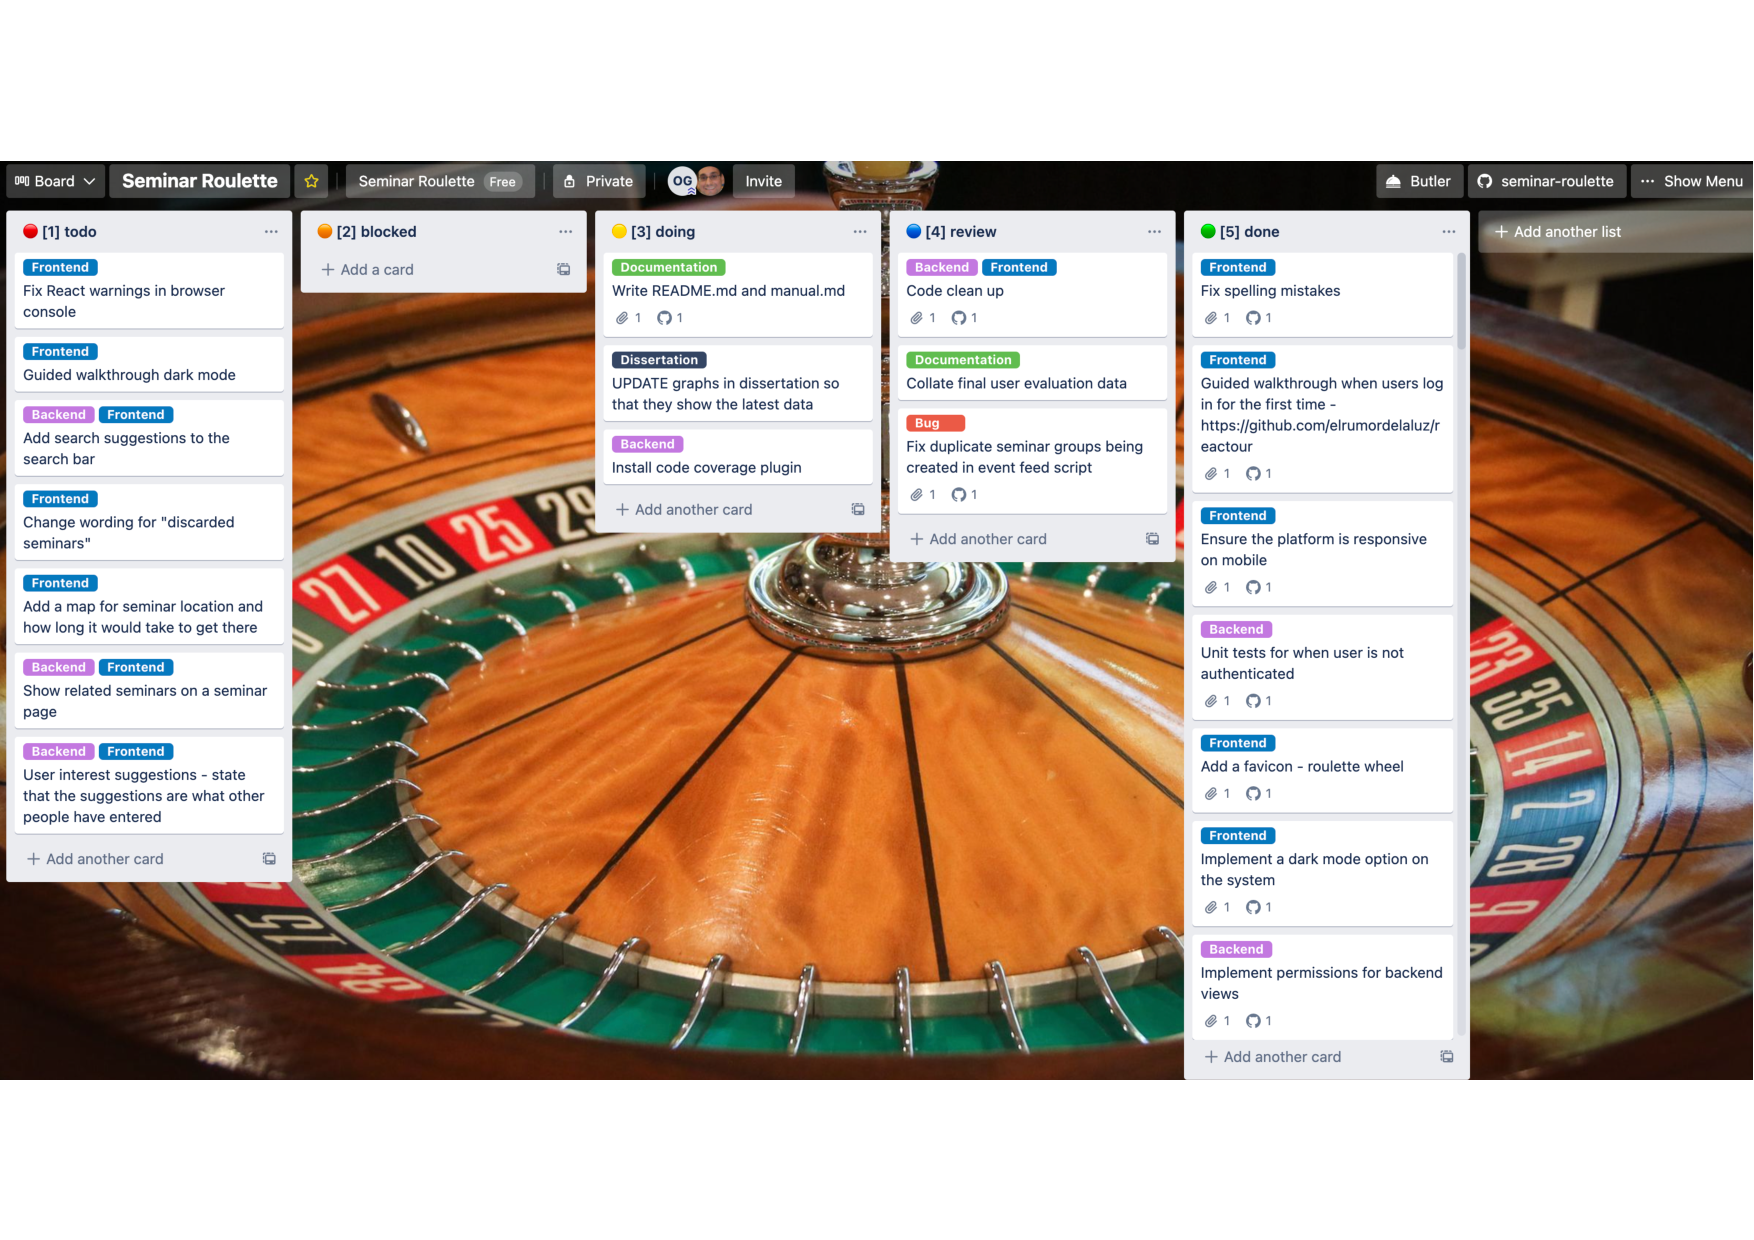
\includegraphics[width=0.9\linewidth]{images/trello_board.pdf}    
    \caption{Seminar Roulette's Trello board, used to split up the project's tasks into various lists corresponding to their current progress.}
    \label{fig:trello_board} 
\end{figure}

\subsection{Kanban Development}

As outlined in Section \ref{section:issue_management}, a Kanban board was created using Trello. Due to the development team only consisting of one person, a Kanban approach was taken towards the development methodology. One of the advantages of using Kanban was that the project could quickly adapt to changing priorities as tasks could be moved effortlessly between the different progress lists when required. This allowed for the list of functional and non-functional requirements devised in Sections \ref{section:functional_requirements} and \ref{section:non_functional_requirements} to evolve naturally and be re-prioritised if required. The release methodology of this technique was to deploy new features whenever they were ready, without the need for fixed timescales. Due to there being no prescribed release times or dates, documentation was created weekly, identifying the issues that had been completed since the previous week.

\section{Tools and Technologies}
\label{section:tools_and_technologies}

Seminar Roulette was built using many tools and technologies. This section will explore these in detail, explain why they were chosen and reflect on whether they were fit for purpose. The chosen technologies build on top of the design work in Chapter \ref{chapter:design}, showing how Seminar Roulette was implemented using one set of technologies.

\subsection{Frontend}

From the outset, it was established that the user interface must be efficient, user friendly and visually pleasing. To satisfy these requirements, React, a JavaScript framework for building user interface components was used \citep{react}. React was chosen as it is open-source and has a large community backing it. It was developed by Facebook and is highly efficient with updating its components when data is changed, ensuring that the latest information was always rendered on Seminar Roulette. React allowed for reusable components to be created - essential in developing the system to the standard illustrated by the high-fidelity prototypes in Section \ref{section:high_fidelity_prototypes}. Components were reused multiple times throughout the platform, for example, the seminar card, loading spinners, filters and pagination.

Another advantage of using React was how it handles state management. It allows for variables to be stored as states, resulting in components having the ability to be updated without reloading the entire page. For example, in Seminar Roulette, if a user chooses to filter or sort seminars, the React components are dynamically updated without a page refresh. This was key as the platform displayed dynamic content that changed frequently. A diagram illustrating React's component lifecycle is shown in Figure \ref{fig:react_life_cycle}.

\begin{figure}[htb]
    \centering
    \includegraphics[width=0.35\linewidth]{images/react_life_cycle.pdf}    
    \caption{Lifecycle of React's components, adapted from \cite{reactlifecycle}.}
    \label{fig:react_life_cycle} 
\end{figure}

To create a consistent user interface and experience, Material-UI, an open-source React UI framework was used to style the site \citep{material-ui}. Material-UI was built using Material Design principles \citep{materialdesign} - a set of guidelines created by Google to help developers build consistent and high-quality applications. Using pre-made frontend components sped up development time as custom components did not have to be designed and implemented. Furthermore, Material-UI contained in-built functionality for handling varying screen sizes, imperative to ensure that the system was compatible on desktop, tablet and mobile. The framework handled this by using responsive user interface elements that adapted to any screen size.

Overall, there were no significant issues with the chosen frontend technologies, and all were fit for purpose. However, in future iterations of Seminar Roulette, a different frontend framework may have to be considered to ensure that the web application can be developed with ease. React has a high development pace, and its environment is constantly being updated. Whilst this could be perceived as an advantage, it impacts the learning curve of React negatively. Furthermore, documentation is sparse and not kept up to date with the constant updates, which could cause problems if Seminar Roulette's development team was to be expanded to multiple developers.

\subsection{Backend}

Django was used to develop the backend of the web application. Django is an open-source Python-based web framework that is free to use \citep{django}. It was chosen due to it being fast, secure, scalable and versatile. It can scale to large amounts of traffic, which was imperative in satisfying requirement \emph{\ref{non_functional_requirement:scale_large_number_users}}, enabling the system to be used by tens of thousands of people. Furthermore, Django is highly secure and prevents developers from being susceptible to SQL injections, cross-site request forgery and cross-site scripting attacks. 

Django's architecture follows a model-view-controller styled pattern. In this project, this architecture was inappropriate due to the system being designed using a three-tier architecture as outlined in Section \ref{section:system_architecture}. This required the frontend and backend to communicate with each other using RESTful API calls. To address this problem, the Django REST Framework (DRF) was used \citep{djangorestframework}, enabling a web API to be created with Python and Django.

The chosen backend technologies were fit for purpose, resulting in a smooth implementation stage and a final prototype to be built successfully. However, if the application were to be built again, Flask would be used. Flask is another Python web framework and is referred to as a microframework as it does not require any external libraries \citep{flask}. It is more lightweight than monolithic Django, and web API's are supported straight out of the box, whereas Django requires the Django REST Framework to be installed. In addition, Flask is used by reputable companies such as Netflix and Reddit \citep{flaskcompanies}, making it a solid choice for the backend framework.

\subsection{Database}

As explained in Section \ref{section:database_design}, a relational database was more appropriate than a NoSQL database to store site and user information. PostgreSQL was chosen as Seminar Roulette's database management system and is also free and open-source \citep{postgresql}. PostgreSQL was favoured over MySQL due to it being better for production-ready systems, crucial if Seminar Roulette was to be deployed as a web service to the University's seminar community. In addition, it has faster read/write speeds which were crucial to the success of system requirement \emph{\ref{non_functional_requirement:response_times}}.

As data was collected, it was stored in a GDPR compliant way, ensuring that a minimal amount of personally identifying information was kept and that database requirement \emph{\ref{non_functional_requirement:gdpr}} was met. The University's checklist for databases storing personal data (see requirement \emph{\ref{non_functional_requirement:gdpr}}) was strictly adhered to. If Seminar Roulette were to be deployed for public use, a privacy policy would be created so that users are aware of what personal data is being kept on them. Furthermore, there would be an option for academics to have their information removed from the database if they wish. Finally, data would not be stored longer than necessary.

PostgreSQL did not cause any issues throughout the project and was suitable for storing relational data. In future iterations of this work, a hybrid structure could be introduced, consisting of both a relational and NoSQL database in a single instance. This would benefit the application as the system would become highly flexible and perform better when retrieving and storing data.

\subsection{User Authentication}

To meet requirement \emph{\ref{functional_requirement:single_sign_on}}, the University's single sign-on was integrated to allow users to authenticate themselves using their GUID and password (see Figure \ref{fig:shibboleth}). The authentication used Shibboleth, a single sign-on architecture that allows people to login to various systems using one set of credentials \citep{shibboleth}. Shibboleth was only present on the deployed version of Seminar Roulette as it needs to run on a Linux virtual machine to function. Further details regarding the deployment process are discussed in Section \ref{section:deployment}. Within the local environment, a fake user was created so that the system could be robustly tested.

\begin{figure}[htb]
    \centering
    \includegraphics[width=0.45\linewidth]{images/shibboleth.pdf}    
    \caption{University's single sign-on, enabling academics to sign in using one identity.}
    \label{fig:shibboleth} 
\end{figure}

Requirement \emph{\ref{functional_requirement:use_system_anonymously}} states that the platform should be able to be used by users who are not authenticated. This was developed on Seminar Roulette to allow academics to browse and search for events happening at the University casually. If users decided to use the system anonymously, their feature set was limited, and access to recommendation features was restricted. Furthermore, they were unable to rate past seminars. This was due to these features all requiring the user's personal information to be stored; for example, if a user rated a seminar five stars, then the database had to store who rated that event.

\section{Recommender Algorithms}
\label{section:recommender_algorithms}

This section outlines the implementation of the algorithms described in Section \ref{section:algorithms}, showing how they were written with the chosen programming language, Python. External libraries used will also be outlined and shown how they were integrated to ensure that the algorithms produced the correct results. 

\subsection{Seminar Recommendations}

Seminar recommendations were provided to users through the Matrix Factorisation via Singular Value Decomposition (SVD) algorithm discussed in Section \ref{section:matrixfactorisationviasvd}. To achieve this, a Python data analysis and manipulation library called Pandas was used \citep{pandas}. This enabled seminar data and user ratings to be turned into a DataFrame, a two-dimensional and size-mutable data structure exclusive to Pandas. DataFrames can be manipulated into matrices to allow the SVD to take place. To handle the SVD, the pre-written \emph{svds} function from SciPy was used. SciPy is a Python package used to solve scientific and mathematical computing problems \citep{scipy}.

\subsection{Similarity Matching}

This section provides a visualisation of the WuPalmer similarity algorithm explored in Section \ref{section:wupalmer}. Figure \ref{fig:seminar_card} displays a seminar titled \emph{The Road to a Sufficiently Smart Compiler}. The system successfully identified the keywords for this talk and displayed them in the bottom right-hand corner - \emph{compilers}, \emph{work} and \emph{specialisation}. The WuPalmer algorithm has calculated that between these keywords and the user's personal interests, there is an 82\% match. In this example, the user's interests are \emph{maths}, \emph{code} and \emph{machine learning}. As expected, there is a reasonably high similarity between these sets of words as \emph{code} and \emph{machine learning} are highly related to \emph{compilers}.

\begin{figure}[htb]
    \centering
    \includegraphics[width=0.8\linewidth]{images/seminar_card.pdf}    
    \caption{A seminar card displaying its keywords and the similarity match based on a user's interests.}
    \label{fig:seminar_card} 
\end{figure}

The WuPalmer algorithm was implemented using the Python Natural Language Toolkit or NLTK for short \citep{nltk}. NLTK is a Python package that contains a suite of libraries for semantic natural language processing. Within NLTK's wordnet library, the pre-written function \emph{wup\_similarity} was used to compute a similarity score between two words.

\subsection{Performance Regressions}
\label{section:performance_regressions}

Throughout the implementation stage of the project, a struggle was ensuring that the recommender algorithm performed efficiently and returned data within an acceptable timeframe. Due to the algorithm being extremely accurate and calculating new seminar suggestions each time the user loaded the main page, it was sometimes slow to execute. It was decided that these inefficiencies were sound for a prototype but would not be suitable for a production system. In the prototype version of the system, accuracy was favoured over performance because the project was limited in time and resources. In future iterations of Seminar Roulette, performance regressions would have to be addressed. A solution to this would be to cache some of the recommendation data, resulting in event suggestions being retrieved from memory if the user has not rated any new seminars when the page is loaded. Another workaround would be to use asynchronous calls so that the user can still browse the rest of the application whilst their recommendations are being calculated. Alternatively, seminar suggestions could be devised using precomputation and updated infrequently. For example, a time-based job scheduler could be set up to calculate event recommendations on a nightly basis, resulting in the system becoming more efficient as it would not have to determine recommendations each time a user loads the site.

\section{Deployment}
\label{section:deployment}

As a Kanban style of development was undertaken for the project's duration, it was imperative that Seminar Roulette was deployed early on and new updates released frequently. The system was deployed to the CentOS distribution of a Linux virtual machine with an Apache web server. The virtual machine used belonged to the University, so the application sat behind the University's firewall. CentOS was chosen as it was one of the operating systems compatible with the University's single sign-on. This caused some significant difficulties, ensuring that the correct version of the requirements was installed and did not conflict with each other. Furthermore, the firewall slowed development time immensely as workarounds had to be found to bypass the firewall at specific points. For example, an SSL certificate could not be signed by an external party to ensure that user data was encrypted during transit when using the system.

When a feature was completed and tested, it was released immediately as per the Kanban development methodology. This process was tedious as it was not automated and had to be done manually. This involved logging into the virtual machine, pulling the latest commit from GitHub, installing any new requirements, migrating the database models, collecting the static files and lastly, restarting the web server. In future, a new continuous integration pipeline would be configured to handle automatic deployment whenever code is merged into the master branch.

In the weeks leading up to the completion of this work, the University had an unexpected power outage in their server room. Unfortunately, this affected Seminar Roulette's virtual machine and resulted in it becoming corrupted and unrecoverable. Due to the upcoming project deadline, there was no time for Seminar Roulette to be set up on a new virtual machine as the deployment process was lengthy. To ensure fast and efficient deployment in the future, Docker \citep{docker} containers could be set up to ensure that Seminar Roulette can be successfully deployed on any machine. This would allow for all of the project's software, libraries and configuration files to be bundled into one and deployed from anywhere in the world, removing the need to install packages and requirements whenever Seminar Roulette has to be installed onto a new virtual machine.

\section{Final Product}

Figure \ref{fig:final_product} on page \pageref{fig:final_product} illustrates the Seminar Roulette system after implementation had been completed. The look of the user interface differs slightly from the high-fidelity prototypes created in Section \ref{section:high_fidelity_prototypes} due to feedback received in a think-aloud evaluation. This will be explored further in Chapter \ref{chapter:evaluation}. Pictured are the various components of Seminar Roulette, allowing seminar attendees to find events with ease that they have not thought about attending before.
 
\begin{figure}[htb] 
    \centering
    \begin{subfigure}[b]{\textwidth}
        \includegraphics[width=\textwidth]{images/final_recommendations.pdf}
        \caption{Seminar Roulette's main page, showing a user's seminar recommendations.}
        \label{fig:final_recommendations}
    \end{subfigure}
    \\[2ex]
    \begin{subfigure}[b]{0.49\textwidth}
        \includegraphics[width=\textwidth]{images/final_past_seminars.pdf}
        \caption{Past seminars, showing the ability to give an event a star rating.}
        \label{fig:final_past_seminars}
    \end{subfigure}
    ~
    \begin{subfigure}[b]{0.49\textwidth}
        \includegraphics[width=\textwidth]{images/final_seminar_expanded.pdf}
        \caption{Expanded seminar, displaying more information about the event.}
        \label{fig:final_seminar_expanded}
    \end{subfigure}
    \\[2ex]
    \begin{subfigure}[b]{0.49\textwidth}
        \includegraphics[width=\textwidth]{images/final_search_results.pdf}
        \caption{Seminars returned following a search for "systems".}
        \label{fig:final_search_results}
    \end{subfigure}
    ~
    \begin{subfigure}[b]{0.49\textwidth}
        \includegraphics[width=\textwidth]{images/final_dark_mode.pdf}
        \caption{Upcoming seminars in dark mode.}
        \label{fig:final_dark_mode}
    \end{subfigure}
    ~
    \caption{Screen captures of the final product after implementation was completed. Figures \subref{fig:final_recommendations} to \subref{fig:final_dark_mode} show the different components of the web application. The layout of the page stays consistent throughout the various views. The user has the option of filtering down the returned seminars using filters. One can filter by time frame, whether the seminar serves refreshments or if the seminar is online or in-person. The list of seminars can also be sorted alphabetically or by start date and time.}
    \label{fig:final_product}
\end{figure}

\section{Summary}

This chapter described the implementation stage of the project, highlighting the various steps that were undertaken to develop the prototype application. The project's organisation was detailed through the use of various Agile software engineering practices. The technologies and libraries used to implement the system were discussed in detail and evaluated based on their suitability. Finally, a high-level overview of the deployment process was provided, enabling another developer to release Seminar Roulette if desired.

%==================================================================================================================================
\chapter{Evaluation} 
\label{chapter:evaluation} 

This chapter provides an evaluation of the Seminar Roulette web application, examining the various complementary approaches undertaken to determine the project's success. These approaches range from assessing the performance of the system and codebase in Sections \ref{section:unit_testing} and \ref{section:system_performance} to evaluations conducted with human participants towards the end of the project in Sections \ref{section:think_aloud_evaluation} and \ref{section:user_evaluation}. To conclude, the functional and non-functional requirements devised in Sections \ref{section:functional_requirements} and \ref{section:non_functional_requirements} will be analysed to determine whether the final prototype satisfied each.

Evaluations that involved human participants adhered to the ethics checklist created by the University's School of Computing Science. Before these took place, the ethics form was signed by both the evaluator and project supervisor, as shown in Appendix \ref{appendix:ethics}.

\section{Unit Testing}
\label{section:unit_testing}

As discussed in Section \ref{section:continuous_integration}, a continuous integration pipeline was configured at the start of the project. It was responsible for running a suite of 42 unit tests whenever code was merged into either the development or master branch. This test suite consisted of 34 backend and eight frontend tests. These tests were created to validate that each of Seminar Roulette's components was performing as intended. The backend unit tests ranged from testing the connection to the Samoa Events API to determining if a seminar filter worked correctly. The Python Coverage library \citep{pythoncoverage} was used to produce a code coverage report, as shown in Table \ref{tab:code_coverage}. The report indicates that an overall coverage of 87\% was achieved by the backend unit tests. Research conducted by \cite{GEORGE2004337} states that a code coverage of between 80\% and 90\% is accepted as the industry standard. Therefore, Seminar Roulette's backend test suite was effective in ensuring that the application performed as expected.

\begin{table}[htb]
    \caption{Code coverage report generated from Python's Coverage library, indicating a total coverage of 87\%.}\label{tab:code_coverage}
    \centering
    \resizebox{0.85\textwidth}{!}{%
    \begin{tabular}{@{}lrrrr@{}}
    \toprule
    \textbf{Module}                 & \textbf{Statements} & \textbf{Missing} & \textbf{Excluded} & \textbf{Coverage} \\ \midrule
    backend/\_\_init\_\_.py         & 1                   & 0                & 0                 & 100\%             \\
    backend/admin.py                & 29                  & 0                & 0                 & 100\%             \\
    backend/apps.py                 & 13                  & 0                & 0                 & 100\%             \\
    backend/managers.py             & 28                  & 5               & 0                 & 82\%              \\
    backend/models.py               & 87                  & 3                & 0                 & 97\%              \\
    backend/serializers.py          & 32                  & 0                & 0                 & 100\%             \\
    backend/tests.py                & 156                 & 0                & 0                 & 100\%             \\
    backend/urls.py                 & 7                   & 0                & 0                 & 100\%             \\
    backend/views/views\_misc.py    & 31                  & 1                & 0                 & 97\%              \\
    backend/views/views\_seminar.py & 142                 & 32               & 0                 & 77\%              \\
    backend/views/views\_user.py    & 107                 & 40               & 0                 & 63\%              \\ \midrule
    \textbf{Total}                  & \textbf{633}        & \textbf{81}      & \textbf{0}        & \textbf{87\%}     \\ \bottomrule
    \end{tabular}%
    }
\end{table}

Along with the backend unit tests, a small suite of eight frontend tests was developed to verify that Seminar Roulette's React components were being rendered correctly to the user. Only a small number of frontend tests were created due to the time constraints of the project. In addition, priority was given to the backend unit tests as these were responsible for testing the underlying logic of the platform and ensuring no broken code was ever pushed to production. The frontend test suite used smoke tests to ensure that the production version of Seminar Roulette was stable enough to be released. An example of an integrated smoke test is shown in Listing \ref{lst:app_smoke_test} to ensure that the application rendered without throwing any errors when the app component was mounted. 

\begin{lstlisting}[language=JavaScript, caption={Frontend smoke test verifying that the app component rendered without crashing or throwing any errors.}, label=lst:app_smoke_test]
    import React from "react";
    import { render, unmountComponentAtNode } from "react-dom";
    import App from "../App";
    
    it("Renders application without crashing", () => {
      const root = document.createElement("div");
      render(<App />, root);
      unmountComponentAtNode(root);
    });
\end{lstlisting}

Along with the eight frontend tests, the frontend was also tested manually through the final user evaluation described in Section \ref{section:user_evaluation}. Although this hybrid of automated and manual frontend testing was sufficient for this project, it was not the most optimal method of testing the user interface. This would have to be addressed in future iterations of the system to ensure that the entirety of the application is tested robustly and automatically.

\section{System Performance}
\label{section:system_performance}

In Section \ref{section:non_functional_requirements}, system requirement \emph{\ref{non_functional_requirement:response_times}} states that the application must be efficient and respond within two seconds. To evaluate this metric, the quality of the application was measured through Lighthouse \citep{lighthouse}, a tool developed by Google that evaluates the performance of websites. Lighthouse is commonly used on commercial websites and measures various metrics, of which five were tracked for this evaluation. These were \emph{performance}, \emph{accessibility}, \emph{best practices}, \emph{time to interactive} and \emph{speed index}. \emph{Time to interactive} was the number of seconds taken for a page to load completely, whilst \emph{speed index} measured the number of seconds it took for a page's contents to be populated visibly. The aforementioned metrics were tracked on each of Seminar Roulette's four pages:

\begin{itemize}
    \item \textbf{Anonymous:} the homepage with a limited feature set available due to the user not being logged in.
    \item \textbf{Single sign-on:} the University's single sign-on page integrated with Shibboleth.
    \item \textbf{Homepage:} the main page of the site when the user has logged in, resulting in all seminar recommendation features being available to them.
    \item \textbf{Search:} the page that appears after a user performs a free-text search for an event.
\end{itemize}

The results from the system performance evaluation are shown in Table \ref{tab:lighthouse_results}. To retrieve these results, the system performance evaluation was carried out three times on the same device and network, with the average score of each metric then being calculated.

\begin{table}[htb]
    \caption{System performance results from Lighthouse's evaluation. The performance, accessibility and best practices columns have a maximum score of 100. Red indicates a poor score. Orange represents that the metric needs improved, and green demonstrates a good score.}\label{tab:lighthouse_results}
    \centering
    \resizebox{0.9\textwidth}{!}{%
    \begin{tabular}{@{}cccccc@{}}
    \toprule
    \textbf{Page}      & \textbf{Performance}       & \textbf{Accessibility}    & \textbf{\makecell{Best \\Practices}}    & \textbf{\makecell{Time to \\Interactive (s)}} & \textbf{\makecell{Speed \\Index (s)}}   \\ \midrule
    Anonymous & {\color[HTML]{009901} 90}  & {\color[HTML]{F56B00} 82} & {\color[HTML]{009901} 93}  & {\color[HTML]{009901} 1.5}       & {\color[HTML]{F56B00} 1.3} \\
    Single sign-on     & {\color[HTML]{009901} 100} & {\color[HTML]{F56B00} 68} & {\color[HTML]{009901} 100} & {\color[HTML]{009901} 0.4}       & {\color[HTML]{009901} 0.4} \\
    Homepage           & {\color[HTML]{F56B00} 59}  & {\color[HTML]{F56B00} 84} & {\color[HTML]{009901} 93}  & {\color[HTML]{F56B00} 2.7}       & {\color[HTML]{CB0000} 3.0} \\
    Search             & {\color[HTML]{F56B00} 60}  & {\color[HTML]{F56B00} 84} & {\color[HTML]{009901} 93}  & {\color[HTML]{F56B00} 3.1}       & {\color[HTML]{F56B00} 1.3} \\ \bottomrule
    \end{tabular}%
    }
\end{table}

Overall, Seminar Roulette functioned well in the performance evaluation. However, there were a few areas where the system scored poorly and will need to be improved. A common trend in the results was that the application performed worse on pages that contained lots of dynamic content. Similarly, pages with fewer features were much more efficient and responded quicker. To determine the success of requirement \emph{\ref{non_functional_requirement:response_times}}, the \emph{time to interactive} metric was analysed as this represented when the page was able to be fully interactive to the user. Based on this, two out of the four pages failed to meet requirement \emph{\ref{non_functional_requirement:response_times}} as they took longer than two seconds to load completely. The pages likely took longer than two seconds to load due to the performance regressions discussed in Section \ref{section:performance_regressions}. The anonymous homepage and single sign-on both passed this test. However, those pages were limited in features and did not represent the system as a whole. Therefore, requirement \emph{\ref{non_functional_requirement:response_times}} was not met, potentially resulting in users becoming deterred from the system and never using it again. Moving forward, the performance regressions would need to be addressed, aiming to reduce page load times to less than two seconds.

\section{Think-Aloud Evaluation}
\label{section:think_aloud_evaluation}

At the end of semester one, a think-aloud evaluation was conducted with six participants: the project supervisor's postgraduate students. All were regular research seminar attendees, and so were a suitable target group to participate. This evaluation aimed to determine the features that they thought were missing from the system at that stage in time. Furthermore, feedback was sought on the user interface and experience to ensure that Seminar Roulette was easy to use without any prior training.

During the evaluation, participants were each interviewed on Zoom for 30 minutes. They were given access to Seminar Roulette and allowed to freely roam the system with no formal tasks to complete. They were asked to speak their thoughts out loud and comment on the usability of the application and whether there were any features that they thought were missing. The feedback received from the think-aloud evaluations is summarised below:

\begin{itemize}
    \item Participants generally found the grid structure of seminars confusing and felt that there was too much information crammed onto the page. This design is illustrated by the high-fidelity prototypes in Figure \ref{section:high_fidelity_prototypes}. Users stated that they would prefer to be greeted with a list of seminars.
    \item Add the ability to filter out seminars that are titled \emph{TBA}, \emph{TBC} or \emph{TBD}.
    \item Be able to see which seminars friends are clicking on and the ones that they are rating highly.
    \item Participants suggested adding a legend or tooltip for the icons to explain what they were representing.
    \item At first glance, the random seminar floating action button was not prominent and in an unexpected place.
    \item Implement the ability to add a seminar to one's calendar.
    \item Some participants reported that they did not understand what the aim of the application was at first and suggested adding some helper text somewhere near the top of the page.
    \item When a seminar was clicked, participants suggested opening the seminar information as a pop-up would be better than taking the user to a new page.
\end{itemize}

The feedback gathered was used to determine how the second semester of the project should be spent. Following the completion of the think-aloud evaluations, attention was turned to the frontend and layout of the system. Action was taken to improve the user interface and experience in semester two.

\section{Final User Evaluation}
\label{section:user_evaluation}

Throughout this work, feedback from human subjects was imperative to ensure that Seminar Roulette fulfilled all of its requirements. Towards the end of the project, a final user evaluation was carried out to measure the suitability and usability of the system. The evaluation collected both quantitative and qualitative data intending to improve the prototype in future iterations further. The final user evaluation was completed by 34 participants.

\subsection{Evaluation Procedure}
\label{section:evaluation_procedure}

As shown in Appendix \ref{appendix:final_evaluation_questionnaire}, a questionnaire was created using Google Forms and was split into three sections - tasks to complete, quantitative data and qualitative data.

\textbf{Tasks to Complete}

Participants were given a list of 10 tasks to perform on Seminar Roulette, enabling them to become familiar with the platform and learn how it functioned. The 10 tasks are listed below:

\begin{enumerate}
    \item Navigate to \url{https://howard.dcs.gla.ac.uk/} in your web browser.
    \item The platform can be used without signing in but has a limited feature set. Please take a look at upcoming and random seminars.
    \item Login using your University of Glasgow GUID and password by clicking the LOGIN button in the navigation bar.
    \item Enter up to five of your personal interests.
    \item Find an upcoming seminar and click on it to discover more information about it.
    \item Filter and sort the seminars to your desired needs.
    \item Find at least two past seminars and rate them.
    \item Navigate to your seminar recommendations.
    \item Find a random seminar.
    \item Search for a seminar.
\end{enumerate}

Following the completion of these tasks, participants were asked to move onto the quantitative data stage of the form.

\textbf{Quantitative Data}

The quantitative data section of the questionnaire was based on a Post-Study System Usability Questionnaire (PSSUQ), a standard method of measuring user satisfaction with a software product \citep{pssuq}. The PSSUQ survey consisted of 16 questions with a seven-point Likert scale ranging from \emph{strongly agree} to \emph{strongly disagree} as the options for responses. Participants were also able to leave a question blank to indicate that it was not applicable. The questions in the PSSUQ survey are shown in Figures \ref{fig:final_evaluation_2} to \ref{fig:final_evaluation_6}.

To determine the overall result of the PSSUQ survey, the scores from the seven-point Likert scale were averaged. The aim was to have as low a score as possible as this indicated good user performance and satisfaction. The advantage of using PSSUQ was that the results could be split up into three subsets, measuring \emph{system usefulness}, \emph{information quality} and \emph{interface quality}. This enabled the usability of each system component to be assessed independently of the other.

\textbf{Qualitative Data}

After completing the PSSUQ survey, participants were asked to fill in a series of open-ended questions. These were designed to elicit qualitative feedback from participants. The questions asked revolved around discovering how users felt Seminar Roulette could be improved in the future or if there were any additional features that they would like added to the system. Furthermore, the qualitative section allowed participants to report bugs and errors that they encountered whilst testing the platform.

\subsection{Quantitative Results}

The PSSUQ aimed to achieve the lowest score possible, where a score of one indicated that the system was easy to use, and seven implied that the platform performed poorly. Seminar Roulette scored 1.9 in the overall PSSUQ, showing that the system was highly usable. As mentioned in Section \ref{section:evaluation_procedure}, the advantage of using a PSSUQ survey was that the overall score could be split into three sub-scores; system usefulness, information quality and interface quality. The results of these were 1.7, 2.0 and 2.0, respectively.

As all three sub-scores were low, the platform was labelled highly usable in usefulness, information quality and interface quality. Based on these scores, non-functional requirements \emph{\ref{non_functional_requirement:no_prior_training}} and \emph{\ref{non_functional_requirement:intuitive_user_interface}} were satisfied as the system was easy to use without any prior training and provided an intuitive user interface. This is further backed up by Figure \ref{fig:simple_system_responses}, where a column chart is shown of user responses to the statement \emph{it was simple to use this system}. 56\% of participants stated that they \emph{strongly agree} that the platform was simple to use.

\begin{figure}[htb] 
    \centering
    \begin{subfigure}[b]{0.43\textwidth}
        \includegraphics[width=\textwidth]{images/simple_system_responses.pdf}
        \caption{PSSUQ quantitative results for question two.}
        \label{fig:simple_system_responses}
    \end{subfigure}
    ~
    \begin{subfigure}[b]{0.47\textwidth}
        \includegraphics[width=\textwidth]{images/system_error_messages.pdf}
        \caption{PSSUQ quantitative results for question seven.}
        \label{fig:system_error_messages}
    \end{subfigure}
    ~
    \caption{Column charts showing participant responses on the seven-point Likert scale where 1 represents "strongly agree", and 7 indicates "strongly disagree". \subref{fig:simple_system_responses} shows responses to the statement "it was simple to use this system", whilst \subref{fig:system_error_messages} shows responses to the statement "the system gave error messages that clearly told me how to fix problems".}
    \label{fig:quantitative_result_graphs}
\end{figure}

The PSSUQ resulted in some low usability scores. While it can be concluded that Seminar Roulette was a success in being simple to use, it should also be noted that there might be some bias in the data collected in the final user evaluation. Due to the restrictions imposed by COVID-19, many of the participants in the evaluation were friends or people who personally knew the evaluator. This may have caused some results to be skewed in favour of the evaluator, and this should be taken into account if Seminar Roulette was to be deployed. Post COVID-19, a further evaluation could be conducted with a new group of participants who do not know the evaluator to determine whether the platform would be suitable in the University's portfolio of event software products.

The most varied results from the PSSUQ came from statement seven; \emph{the system gave error messages that clearly told me how to fix problems} (see Figure \ref{fig:system_error_messages}). There were only 14 responses meaning that 20 participants left this statement blank to indicate that it was not applicable. In addition, three participants stated that they \emph{strongly disagree} with the platform displaying error messages to them. This implies that Seminar Roulette could have been better in showing descriptive error messages to users when they encountered problems. By not improving upon this, users could become confused and these issues could deter them from using the application ever again. As only four participants disagreed with this statement, it was deemed that non-functional requirement \emph{\ref{non_functional_requirement:alert_users_to_errors}} was still met as 10 participants gave positive feedback. 

\subsection{Qualitative Results}

After finishing the PSSUQ survey, participants were asked to complete five open-ended questions to elicit qualitative feedback. These questions were designed to further assess the suitability of Seminar Roulette and shaped the future work outlined in Section \ref{section:future_work} of Chapter \ref{chapter:conclusion}. The responses to these five questions have been summarised below.

\textbf{Whilst using Seminar Roulette, did you encounter any errors? If so, please describe the error and how it arose.}

59\% of respondents reported that they did not encounter any errors whilst using the platform, showing that the system is bug free and can reliably provide seminar recommendations to University academics. Bugs that were reported were not detrimental to the functionality of the system. These included minor spelling mistakes and lots of users experiencing slow loading times, further backing up the performance issues discussed in Section \ref{section:performance_regressions}.

\textbf{Do you think that Seminar Roulette could be a useful platform to provide seminar recommendations to university academics? If no, please specify why not.}

All 34 participants said that Seminar Roulette would be a suitable platform to provide seminar recommendations to academics, showing that a desire exists for a system of this nature within the University's software portfolio.

\textbf{Do you have any suggestions on how the Seminar Roulette platform could be improved?}

Many different suggestions were given for how the platform could be improved in the future. The most noteworthy of these were: 

\begin{itemize}
    \item Fix the performance problems so that users do not have to wait a long time to receive their recommendations.
    \item Make the four tabs, \emph{recommendations}, \emph{upcoming}, \emph{past} and \emph{random} clearer as there was occasionally some confusion as to what these were representing.
    \item Some participants did not understand the difference between seminar recommendations and the personal interests percentage matching. Users suggested adding some helper text on the homepage to describe the differences between the two features.
\end{itemize}

\textbf{Are there any additional features that you would like to see in Seminar Roulette?}

There was some overlap between features suggested by participants and features outlined in the functional requirements that were not implemented due to time constraints. The most common future feature suggestions were:

\begin{itemize}
    \item Implement a discussion area where attendees could exchange messages pre and post-event.
    \item Add graphics for the seminar speaker to make it easier to network with people at the event.
    \item Integration with Microsoft Exchange calendar and only recommend seminars that fit around an academic's schedule.
\end{itemize}

\textbf{In five words, how would you describe the overall design and functionality of Seminar Roulette?}

The final question of the user evaluation form asked participants to describe the overall design and functionality of Seminar Roulette in five words. Using their responses, a word cloud was created (see Figure \ref{fig:word_cloud}) to show a weighted list of the most common feedback received. The most common words received were \emph{easy}, \emph{clean}, \emph{simple} and \emph{intuitive}, solidifying the aims set out in Section \ref{sec:aims}. These words were used by respondents 16, 13, 9 and 8 times, respectively.

\begin{figure}[htb]
    \centering
    \includegraphics[width=0.6\linewidth]{images/word_cloud.pdf}    
    \caption{Word cloud displaying words that participants used to describe their experience with Seminar Roulette. The size of each word correlates with the number of times that word was used by participants.}
    \label{fig:word_cloud} 
\end{figure}

\section{Requirement Validation}

To complete the evaluation of Seminar Roulette, the functional and non-functional requirements devised in Sections \ref{section:functional_requirements} and \ref{section:non_functional_requirements} were analysed to determine whether they had been satisfied or not. Within these sections, three requirements were assigned the priority \emph{Won't Have This Time} and were out of the project's scope from the outset. As a result, these requirements will be excluded from this section of the evaluation.

In total, 27 functional and non-functional requirements were considered. Of these, 21 were met or 78\%, as shown in Table \ref{tab:requirement_validation}. All \emph{Must Have} requirements were satisfied apart from \emph{\ref{non_functional_requirement:response_times}} for reasons outlined in Section \ref{section:system_performance}. All five \emph{Should Have} requirements were successfully implemented. None of the five \emph{Could Have} requirements were met due to the time constraints of the project. Not fulfilling these requirements was not detrimental to the final evaluation outcome as they were only going to be implemented if time allowed.

Whilst the final prototype did not deliver on all of the requirements that it set out to achieve, the project was still regarded as a success due to 78\% of all requirements, and 94\% of \emph{Must Have} requirements being satisfied successfully. Future iterations of Seminar Roulette will aim to improve upon this figure, with 100\% requirement satisfaction being the ultimate goal.

\begin{table}[htb]
    \caption{List of functional and non-functional requirements, showing whether the final prototype satisfied the requirement or not and its corresponding priority. A \checkmark signifies that the requirement was met whilst a $\times$ shows that it was not.}
    \label{tab:requirement_validation}
    \begin{subtable}[t]{0.5\linewidth}
        \centering
        \caption{Functional requirements.}
        \begin{tabular}{@{}ccc@{}}
            \toprule
            \textbf{Requirement} & \textbf{Priority} & \textbf{Satisfied} \\ \midrule
            S1                   & MH                & \checkmark         \\
            S2                   & MH                & \checkmark         \\
            S3                   & SH                & \checkmark         \\
            S4                   & CH                & $\times$           \\
            S5                   & CH                & $\times$           \\
            S6                   & WH                & $\times$           \\
            U1                   & MH                & \checkmark         \\
            U2                   & MH                & \checkmark         \\
            U3                   & MH                & \checkmark         \\
            U4                   & MH                & \checkmark         \\
            U5                   & SH                & \checkmark         \\
            U6                   & SH                & \checkmark         \\
            U7                   & SH                & \checkmark         \\
            U8                   & CH                & $\times$           \\
            U9                   & CH                & $\times$           \\
            U10                  & CH                & $\times$           \\
            A1                   & MH                & \checkmark         \\
            A2                   & SH                & \checkmark         \\
            A3                   & WH                & $\times$           \\
            D1                   & MH                & \checkmark         \\
            D2                   & MH                & \checkmark         \\
            D3                   & WH                & $\times$           \\ \bottomrule 
        \end{tabular}
    \end{subtable}
    \begin{subtable}[t]{0.5\linewidth}
        \centering
        \caption{Non-functional requirements.}
        \begin{tabular}{@{}ccc@{}}
            \toprule
            \textbf{Requirement} & \textbf{Priority} & \textbf{Satisfied} \\ \midrule
            S7                   & MH                & \checkmark         \\
            S8                   & MH                & \checkmark         \\
            S9                   & MH                & \checkmark         \\
            S10                  & MH                & $\times$           \\
            S11                  & MH                & \checkmark         \\
            U11                  & MH                & \checkmark         \\
            U12                  & MH                & \checkmark         \\
            D4                   & MH                & \checkmark         \\ \bottomrule
            \end{tabular}
    \end{subtable} 
\end{table}

\section{Summary}

This chapter described various evaluation methods in order to determine the success of the final prototype. The range of evaluative techniques measured the robustness of the codebase, time taken for the system to become interactive, multiple user evaluations with human participants and finally validation of the functional and non-functional requirements set out in Sections \ref{section:functional_requirements} and \ref{section:non_functional_requirements}.

%==================================================================================================================================
\chapter{Conclusion}    
\label{chapter:conclusion}

This chapter begins with a reflection in Section \ref{section:reflection} of what went well and what did not within the project, investigating future work that could be undertaken if the project was to be continued for another six months in Section \ref{section:future_work}. Finally, a summary of the entirety of this work is provided in Section \ref{section:summary}.

\section{Reflection}
\label{section:reflection}

This project has allowed the developer to gain a greater insight into the inner workings of University systems and learn how to build clean, responsive and functional user interfaces for deployed software. Another key takeaway from this work was the self-organisation required to develop a large-scale software product single-handedly. Prior to this project, work of this size had only been undertaken by the author in a group setting with multiple developers on board. The iterative nature of this project was new to the developer and allowed for the idea of Seminar Roulette to come to fruition. This took Seminar Roulette from paper prototypes to a robust Django and React web application. The evaluation process of the project was mainly new to the developer, and it allowed them to realise how large-scale software products might be tested and evaluated within industry.

Seminar Roulette acted as the author's first time developing a recommender system within a software product. The developer had to conduct extensive research into the most suitable algorithm for the task and learn how to implement it using the chosen technologies. This was a huge learning curve and took a significant amount of time during the design and implementation stages.

If Seminar Roulette were to be built from scratch again, further initial research would be conducted into how to ensure that the system is accessible to users with impairments, as this is something that was overlooked within the design stage of the project. Furthermore, more attention would be given to the colour scheme and design, ensuring that the platform looks and feels like a University software product.

\section{Future work}
\label{section:future_work}

A multitude of work could be undertaken to extend the functionality of Seminar Roulette in the future. However, before additional features could be implemented, the short-term goal would be to address the current performance issues to ensure that the platform is efficient as possible. In turn, this would improve usability and reduce the likeliness of the platform becoming cumbersome to use.

For future implementation, the functional and non-functional requirements identified in Sections \ref{section:functional_requirements} and \ref{section:non_functional_requirements} that were not achieved would be prioritised. As none of the \emph{Could Have} requirements were implemented, these would be acted upon first. The main focus would involve extending the functionality of the recommendation feature, allowing academics to connect their Microsoft Exchange calendar to Seminar Roulette to enable seminar suggestions to be made that fit around their timetable. This would allow users to have an even more personalised experience with the system.

Although the prototype in its current state scrapes data from Samoa Events and Eventbrite, the University of Glasgow use other services to advertise seminars taking place on campus. These feeds were not included in the database population script discussed in Section \ref{section:database_population_script} due to the time constraints of the project. Other data feeds that could be integrated into Seminar Roulette are Bookitbee \citep{bookitbee}, Yammer \citep{yammer} and Meetup \citep{meetup}. Bookitbee is an online booking system for events. Yammer is a social networking platform used within large organisations, and Meetup is an online service to organise events. Whilst Bookitbee and Yammer both have their own pages exclusive to the University, Meetup is an external platform that would allow Seminar Roulette to extend its functionality to show events happening in Glasgow but outwith the University.

In future iterations of Seminar Roulette, the platform could be re-targeted for other academic institutions, allowing other Universities to provide their academics with event recommendations. The current application is closely coupled to University of Glasgow business systems. A new version of the platform would have to re-target the single sign-on and database population script to the relevant data feeds. This process is better known as \emph{white labelling}, where a product is produced that has the capability to be re-branded to suit any requirements. For example, if the University of Strathclyde wanted to add Seminar Roulette to their software portfolio, the database population script would need to include their event data feeds. Strathclyde advertises seminars through their website and their own custom seminar system, sbs.strath \citep{sbs.strath}.

\section{Summary}
\label{section:summary}

In summary, Seminar Roulette is a web-based platform designed to provide event recommendations to University of Glasgow academics. The system has successfully managed to pull in data from both Samoa Events and Eventbrite, enabling it to become a centralised hub for seminar attendees. Users can rate past seminars and enter keywords that relate to their personal interests. In response, users are provided with a list of event recommendations and a percentage value for how similar a seminar is to their interests. The system made use of the University's single sign-on, allowing academics to login to the application using their University GUID and password.

Seminar Roulette was evaluated using various techniques, including unit testing, system performance, two end-user evaluations and requirement validation. Using the aforementioned methods, it was concluded that Seminar Roulette effectively provides valuable seminar suggestions to members of the University's academic community. Although the system had some significant performance issues, the platform was still deemed highly usable and able to be used without any prior training. By achieving both of these goals, the original aims set out in Section \ref{sec:aims} were validated.

With some minor adjustments, Seminar Roulette, in its current state, could be deployed as a web service within the University of Glasgow, allowing academics to discover seminars and events that they have not thought about attending before. By successfully implementing a working prototype, the platform is the first University system to adopt a unified approach to seminar management. This solidifies the speculation outlined in Section \ref{sec:aims}, where it was stated that \emph{there is potential for the new system to become a staple piece of software in the University's seminar community}. Therefore, the entirety of this work can be regarded as a success.

%==================================================================================================================================
%
% 
%==================================================================================================================================
%  APPENDICES  

\begin{appendices}

\chapter{Ethics Checklist}
\label{appendix:ethics}

This appendix contains a copy of the ethics checklist, required to be signed before end-user evaluations with participants could take place.

\begin{figure}[htb]
    \centering
    \includegraphics[width=0.85\linewidth]{images/signed_ethics_checklist_1.pdf}    
    \caption{Signed ethics checklist - page 1 of 2.}
    \label{fig:signed_ethics_checklist_1} 
\end{figure}

\begin{figure}[htb]
    \centering
    \includegraphics[width=0.85\linewidth]{images/signed_ethics_checklist_2.pdf}    
    \caption{Signed ethics checklist - page 2 of 2.}
    \label{fig:signed_ethics_checklist_2} 
\end{figure}


\chapter{Initial User Survey}
\label{appendix:initial_user_survey}

This appendix provides the initial user survey, which was distributed amongst key stakeholders to build a list of requirements.

\begin{figure}[htb]
    \centering
    \includegraphics[width=\linewidth]{images/initial_user_survey_1.pdf}    
    \caption{Initial user survey - page 1 of 4.}
    \label{fig:initial_user_survey_1} 
\end{figure}

\begin{figure}[htb]
    \centering
    \includegraphics[width=\linewidth]{images/initial_user_survey_2.pdf}    
    \caption{Initial user survey - page 2 of 4.}
    \label{fig:initial_user_survey_2} 
\end{figure}

\begin{figure}[htb]
    \centering
    \includegraphics[width=\linewidth]{images/initial_user_survey_3.pdf}    
    \caption{Initial user survey - page 3 of 4.}
    \label{fig:initial_user_survey_3} 
\end{figure}

\begin{figure}[htb]
    \centering
    \includegraphics[width=\linewidth]{images/initial_user_survey_4.pdf}    
    \caption{Initial user survey - page 4 of 4.}
    \label{fig:initial_user_survey_4} 
\end{figure}


\chapter{Samoa Events API Response}
\label{appendix:samoa_api_response}

This appendix contains an extract of the JSON response returned when the Samoa Events API was called.

\begin{lstlisting}[language=json, caption={Extract of JSON response from Samoa Events API.}]
{
   "id":17712,
   "title":"A usability model for online coding tutorials systems",
   "startTime":"2021-03-09T14:30",
   "endTime":"2021-03-09T15:00",
   "speaker":"Ohud Alasmari",
   "speakerAffiliation":"University of Glasgow",
   "speakerUrl":"https://www.gla.ac.uk/pgrs/ohudalasmari/#supervisors",
    "description":"<p><span>Online Coding Tutorial systems provide a basis for free and open interactive programming education at scale. Such browser-based systems featuring automated feedback are increasingly popular as remote learning has become normalized. Programming students with different social and cultural backgrounds from all over the world can access these platforms. In addition, Online Coding Tutorials facilitate practical software development experiences that form an integral part of the learning process for novice programmers. However, such systems will only be truly effective if they meet diverse programming learner requirements. In this paper, we argue that these requirements must be informed by a range of disciplines, including system usability, computing pedagogy, and internationalization. We conducted a wide-ranging survey of partially relevant usability models; from these studies we synthesized a new and specialized hierarchical usability model for Online Coding Tutorial systems. This new model has four dimensions: pedagogy, platform, culture and cognition. We claim that, in relation to previous models, our multi-dimensional framework covers a more comprehensive range of requirements for online programming language learners. This framework can be used to characterize and compare existing online tools, as well as to inform good design practice for new tools. We provide initial evidence of the potential utility of our model by applying it to three mainstream programming learning tools: LearnPython, TryRuby, and TryJavaScript.</span></p>",
   "location":{
      "id":200,
      "location":"Zoom",
      "directions":"",
      "mapUrl":null,
      "latitude":0.0,
      "longitude":0.0
   },
   "locationId":200,
   "owningOu":{
      "id":27,
      "parent":5,
      "name":"Systems Seminars",
      "url":"https://www.gla.ac.uk/schools/computing/research/
      researchsections/systems-section/",
      "location":1,
      "description":"<p>The GLAsgow Systems Section (GLASS) researches parallel and distributed systems, networked systems and (safety-critical) software systems. We have a strong focus on real-world systems, and cover all scales and across the hardware-software spectrum. We contribute to, develop and release open source research software. There are several research groups within the section:</p>\r\n<ul>\r\n<li><span><a href=\"http://www.dcs.gla.ac.uk/research/gpg/\">GPG: The Glasgow Parallelism Group</a></span><span>&nbsp;(led by Phil Trinder)</span></li>\r\n<li><span><a href=\"http://www.dcs.gla.ac.uk/research/networked-systems/\">
      Networked Systems</a></span>&nbsp;(led by Colin Perkins)</li>\r\n<li><span><a href=\"../../schools/computing/research/researchoverview/
      systemsengineeringresearchgroup/#d.en.481939\">Systems Engineering</a></span><span>&nbsp;(led by Tim Storer)</span></li>\r\n</ul>\r\n<p>Much of the research we undertake is collaborative and has industrial partners. We work closely with other groups in Computing Science as well as other schools including Engineering. We also work closely with other world leading Universities and many private and public sector organisations (recently: Airbus, Cisco Systems, EDF, Ericsson, GCHQ, IETF, Microsoft Research, NASA).</p>\r\n<p>Systems seminars are usually held on Wednesdays. Everyone from the University of Glasgow and beyond is welcome to attend these talks - see the Events tab for more details. We are happy to hear from anyone that would like to visit us to give a talk.</p>\r\n<p>The Systems seminar coordinators are Natalia Chechina and Magnus Morton.</p>",
      "shortname":"socs-systems-seminars",
      "status":"ACTIVE",
   },
   "owningOuId":27,
   "owningGuid":"2426493a",
   "lastModified":"2021-03-03T20:05:35Z",
   "lastModifiedGuid":"2426493a",
   "registrationUrl":"",
   "intendedAudience":0,
   "userActionsAllowed":0,
   "userTagList":[
      "public"
   ],
   "marked":false,
   "extraLocation":null,
   "valid":true
}
\end{lstlisting}


\chapter{Final User Evaluation Questionnaire}
\label{appendix:final_evaluation_questionnaire}

This appendix provides the final user evaluation questionnaire that was used to collect participant's feedback.

\begin{figure}[htb]
    \centering
    \includegraphics[width=\linewidth]{images/final_evaluation_1.pdf}    
    \caption{Final user evaluation questionnaire - page 1 of 8.}
    \label{fig:final_evaluation_1} 
\end{figure}

\begin{figure}[htb]
    \centering
    \includegraphics[width=\linewidth]{images/final_evaluation_2.pdf}    
    \caption{Final user evaluation questionnaire - page 2 of 8.}
    \label{fig:final_evaluation_2} 
\end{figure}

\begin{figure}[htb]
    \centering
    \includegraphics[width=\linewidth]{images/final_evaluation_3.pdf}    
    \caption{Final user evaluation questionnaire - page 3 of 8.}
    \label{fig:final_evaluation_3} 
\end{figure}

\begin{figure}[htb]
    \centering
    \includegraphics[width=\linewidth]{images/final_evaluation_4.pdf}    
    \caption{Final user evaluation questionnaire - page 4 of 8.}
    \label{fig:final_evaluation_4} 
\end{figure}

\begin{figure}[htb]
    \centering
    \includegraphics[width=\linewidth]{images/final_evaluation_5.pdf}    
    \caption{Final user evaluation questionnaire - page 5 of 8.}
    \label{fig:final_evaluation_5} 
\end{figure}

\begin{figure}[htb]
    \centering
    \includegraphics[width=\linewidth]{images/final_evaluation_6.pdf}    
    \caption{Final user evaluation questionnaire - page 6 of 8.}
    \label{fig:final_evaluation_6} 
\end{figure}

\begin{figure}[htb]
    \centering
    \includegraphics[width=\linewidth]{images/final_evaluation_7.pdf}    
    \caption{Final user evaluation questionnaire - page 7 of 8.}
    \label{fig:final_evaluation_7} 
\end{figure}

\begin{figure}[htb]
    \centering
    \includegraphics[width=\linewidth]{images/final_evaluation_8.pdf}    
    \caption{Final user evaluation questionnaire - page 8 of 8.}
    \label{fig:final_evaluation_8} 
\end{figure}

\end{appendices}

%==================================================================================================================================
%   BIBLIOGRAPHY   

% The bibliography style is abbrvnat
% The bibliography always appears last, after the appendices.

\bibliographystyle{abbrvnat}

\bibliography{l4proj}

\end{document}
